\part{Angular Momentum and Spin}
\section{Angular Momentum}
\subsection{Angular Momentum in Classical Mechanics}
In classical mechanics the angular momentum of a particle at position \(\vv{x}\) with momentum \(\vv{p}\) is
\[\vv{L} = \vv{x} \times \vv{p}.\]
As a vector equation this can be written as three scalar equations:
\[L_x = yp_z - zp_y, \qquad L_y = zp_x - xp_z,\qquad\text{and}\qquad L_z = xp_y - yp_x.\]
These can be written more concisely as
\[L_i = \varepsilon_{ijk}x_jp_k\]
where \((x_1, x_2, x_3) = (x, y, z)\) and \((p_1, p_2, p_3) = (p_x, p_y, p_z)\) and \(\varepsilon_{ijk}\) is the Levi-Civita symbol defined as
\[
\varepsilon_{ijk} = 
\begin{cases}
    1, & (i,j,k) = (1, 2, 3), (2, 3, 1), (3, 1, 2),\\
    -1, & (i, j, k) = (1, 3, 2), (2, 1, 3), (3, 2, 1),\\
    0, & \text{otherwise},
\end{cases}
\]
and we have applied the Einstein summation convention of summing over repeated indices.

\subsection{Angular Momentum in Quantum Mechanics}
\subsubsection{Angular Momentum Operators}
Angular momentum is an observable and so has an associated Hermitian operator.
The \define{angular momentum operator} for the angular momentum in the \(\ve{i}\) direction is
\[\operator{L}_i = \varepsilon_{ijk}\operator{X}_j\operator{P}_k.\]
We can write this as a cross product of vectors of operators:
\[\vecoperator{L} = \vecoperator{X}\times\vecoperator{P}.\]
For a state \(\ket{\psi}\in\hilbert\) if we define \(\operator{L}_k\ket{\psi} = \ket{\varphi}\) then
\[\bra{\vv{r}}\operator{L}_k\ket{\psi} = \braket{\vv{r}}{\varphi} = \varphi(\vv{r}) = \operator{L}_k\psi(\vv{r}) = -\hbar\varepsilon_{ijk}x_j\pdv{\psi}{x_k}.\]

\subsubsection{Angular Momentum Commutators}
Since \(\operator{L}_i\) are defined as a product of position and momentum operators we expect the commutation relations between different components of the angular momentum to be non-trivial, for example:
\begin{align*}
    [\operator{L}_x, \operator{L}_y] &= [\operator{Y}\operator{P}_z - \operator{Z}\operator{P}_y, \operator{Z}\operator{P}_x - \operator{X}\operator{P_z}]\\
    &= [\operator{Y}\operator{P}_z, \operator{Z}\operator{P}_x] - [\operator{Z}\operator{P}_y, \operator{Z}\operator{P_x}] - [\operator{Y}\operator{P}_z, \operator{X}\operator{P}_z] + [\operator{Z}\operator{P}_y, \operator{X}\operator{P}_z]\\
    &= [\operator{Y}\operator{P}_z, \operator{Z}\operator{P}_x] - \operator{Z}[\operator{P}_y, \operator{P}_x] - [\operator{Y}, \operator{X}]\operator{P}_z + [\operator{Z}\operator{P}_y, \operator{X}\operator{P}_z]\\
    &= \operator{Y}\operator{P}_z\operator{Z}\operator{P_x} - \operator{Z}\operator{P}_x\operator{Y}\operator{P}_z + \operator{Z}\operator{P}_y\operator{X}\operator{P_z} - \operator{X}\operator{P}_z\operator{Z}\operator{P}_y\\
    &= \operator{Y}\operator{P}_x(\operator{P}_z\operator{Z} - \operator{Z}\operator{P}_z) + \operator{X}\operator{P}_y(\operator{Z}\operator{P}_z - \operator{P}_z\operator{Z})\\
    &= \operator{Y}\operator{P}_x[\operator{P}_z, \operator{Z}] + \operator{X}\operator{P}_y[\operator{Z}, \operator{P}_z]\\
    &= -i\hbar\operator{Y}\operator{P}_x + i\hbar\operator{X}\operator{P}_y\\
    &= i\hbar\operator{L}_z.
\end{align*}
A couple of sanity checks that we can perform here are that \(\operator{L}_k\) is Hermitian so the commutator should be anti-Hermitian, which it is, and also the units of the commutator are angular momentum squared and \(\hbar\) and \(\operator{L}_z\) also both have units of angular momentum so the units match.
Noting that \([\operator{L}_i, \operator{L}_j] = -[\operator{L}_j, \operator{L}_i]\) and \([\operator{L}_i, \operator{L}_i] = 0\) we have that
\[[\operator{L}_i, \operator{L}_j] = i\hbar\varepsilon_{ijk}\operator{L}_k.\]
Since this is non-zero when \(i\ne j\) we see that measuring the angular moment in one direction and then another changes the probability for measuring the angular momentum in the first direction.

\subsubsection{Angular Momentum Differential Operators}
As with the other operators we have introduced we can view \(\operator{L}_i\) as differential operators acting on the wave function.
In this case
\[\operator{L}_x = \varepsilon_{1jk}\operator{X}_j\operator{P}_k = \operator{X}_2\operator{P}_3 - \operator{X}_3\operator{P}_2 = -i\hbar\left(y\pdv{z} - z\pdv{y}\right).\]
Similarly
\[\operator{L}_y = -i\hbar\left(z\pdv{x} - x\pdv{z}\right), \qquad\text{and}\qquad \operator{L}_z = -i\hbar\left(x\pdv{y} - y\pdv{x}\right).\]
Or more compactly
\[\operator{L}_i = -i\hbar\varepsilon_{ijk}x_j\pdv{x_k}.\]
We can use these to derive the commutation relationships that we derived in the last section using the canonical commutation relationship:
\begin{align*}
    \operator{L}_x\operator{L}_y\psi &= -\hbar^2\left(y\pdv{z} - z\pdv{y}\right)\left(z\pdv{x} - x\pdv{z}\right)\psi\\
    &= -\hbar^2\left(y\pdv{z} - z\pdv{y}\right) \left(z\pdv{\psi}{x} - x\pdv{\psi}{z}\right)\\
    &= -\hbar^2\left[y\pdv{z}\left(z\pdv{\psi}{x}\right) - y\pdv{z}\left(x\pdv{\psi}{z}\right) - z\pdv{y}\left(z\pdv{\psi}{x}\right) + z\pdv{y}\left(x\pdv{\psi}{z}\right)\right]\\
    &= -\hbar^2\left[y\pdv{\psi}{x} + yz\pdvsec{\psi}{z}{x} - yx\pdv[2]{\psi}{z} - z^2\pdvsec{\psi}{y}{x} + zx\pdv{\psi}{y}{z}\right]\\
\end{align*}
Similarly
\begin{align*}
    \operator{L}_y\operator{L}_x\psi &= -\hbar^2\left(z\pdv{x} - x\pdv{z}\right)\left(y\pdv{z} - z\pdv{y}\right)\psi\\
    &= -\hbar^2\left(z\pdv{x} - x\pdv{z}\right)\left(y\pdv{\psi}{z} - z\pdv{\psi}{y}\right)\\
    &= -\hbar^2\left[z\pdv{x}\left(y\pdv{\psi}{z}\right) - z\pdv{x}\left(z\pdv{\psi}{y}\right) - x\pdv{z}\left(y\pdv{\psi}{z}\right) + x\pdv{z}\left(z\pdv{\psi}{y}\right)\right]\\
    &= -\hbar^2\left[zy\pdvsec{\psi}{x}{z} - z^2\pdvsec{\psi}{x}{y} - x\pdv[2]{\psi}{z} + xz\pdvsec{\psi}{z}{y} + x\pdv{\psi}{y}\right]
\end{align*}
Hence
\[[\operator{L}_x, \operator{L}_y]\psi = -\hbar^2\left(x\pdv{\psi}{y} - y\pdv{\psi}{x}\right) = i\hbar\operator{L}_z\psi.\]

Angular momentum is often of importance when discussing central potentials, that is potentials of the form \(V(r)\).
It is often best to work spherical coordinates when this is the case:
\begin{align*}
    \operator{L}_x &= i\hbar\left[\sin\varphi \pdv{\vartheta} + \cot\vartheta \cos\varphi \pdv{\varphi}\right],\\
    \operator{L}_y &= i\hbar\left[-\cos\varphi \pdv{\vartheta} + \cot\vartheta \sin\varphi \pdv{\varphi}\right],\\
    \operator{L}_z &= -i\hbar\pdv{\varphi}.
\end{align*}

\subsubsection{Square of the Angular Momentum}
We now introduce the square of the magnitude of the angular momentum:
\[\operator{L}^2 = \operator{L}_x^2 + \operator{L}_y^2 + \operator{L}_z^2 = \sum_{i=1}^{3} \operator{L}_i^2.\]
This can be written as a differential operator in spherical coordinates as
\begin{equation}\label{eqn:L^2 in spherical coord}
    \operator{L}^2 = -\hbar^2 \left[\frac{1}{\sin\vartheta}\pdv{\vartheta}\left(\sin\vartheta \pdv{\vartheta}\right) + \frac{1}{\sin^2\vartheta}\pdv[2]{\varphi}\right].
\end{equation}
Importantly this is compatible with any of the Cartesian components of the angular momentum.
For example,
\begin{align*}
    [\operator{L}^2, \operator{L}_z] &= [\operator{L}_x^2 + \operator{L}_y^2 + \operator{L}_z^2, \operator{L}_z]\\
    &= [\operator{L}_x^2, \operator{L}_z] + [\operator{L}_y^2, \operator{L}_z] + [\operator{L}_z^2, \operator{L}_z]\\
    &= [\operator{L}_x^2, \operator{L}_z] + [\operator{L}_y^2, \operator{L}_z]\\
    &= \operator{L}_x\operator{L}_x\operator{L}_z - \operator{L}_z\operator{L}_x\operator{L}_x + \operator{L}_y\operator{L}_y\operator{L}_z - \operator{L}_z\operator{L}_y\operator{L}_y\\
    &= \operator{L}_x\operator{L}_x\operator{L}_z - \operator{L}_z\operator{L}_x\operator{L}_x + \operator{L}_y\operator{L}_y\operator{L}_z - \operator{L}_z\operator{L}_y\operator{L}_y\\
    &= \operator{L}_x\operator{L}_z\operator{L}_x - \operator{L}_x[\operator{L}_z, \operator{L}_x] + \operator{L}_z\operator{L}_x\operator{L}_x + \operator{L}_y\operator{L}_z\operator{L}_y - \operator{L}_y[\operator{L}_z, \operator{L}_y] - \operator{L}_z\operator{L}_y\operator{L}_y\\
    &= [\operator{L}_x, \operator{L}_z]\operator{L}_x - \operator{L}_x[\operator{L}_z, \operator{L}_x] + [\operator{L}_y, \operator{L}_z]\operator{L}_y - \operator{L}_y[\operator{L}_z, \operator{L}_y]\\
    &= -i\hbar\operator{L}_y\operator{L}_x - i\hbar\operator{L}_x\operator{L}_y + i\hbar\operator{L}_x\operator{L}_y + i\hbar\operator{L}_y\operator{L}_x\\
    &= 0.
\end{align*}
Here we have used
\[\operator{A}\operator{B} - \operator{B}\operator{A} = [\operator{A}, \operator{B}] \implies \operator{B}\operator{A} = \operator{A}\operator{B} - [\operator{A}, \operator{B}]\]
to introduce the first two commutators.
The second two commutators come from factorising.

\subsubsection{Eigenfunctions of \texorpdfstring{\(\operator{L}^2\)}{Lsquared} and \texorpdfstring{\(\operator{L}_z\)}{Lz}}
Since \(\operator{L}^2\) is compatible with all Cartesian components of the angular momentum we know that \(\operator{L}^2\) and \(\operator{L}_z\) must have simultaneous eigenfunctions, and a common eigenbasis.
We work with \(\operator{L}_z\) here as is the convention but all of this holds for \(\operator{L}_x\) and \(\operator{L}_y\) as well.

As with the Harmonic oscillator we will introduce the solution first and discus its properties and derive the solution later.
The simultaneous eigenfunctions of \(\operator{L}^2\) and \(\operator{L}_z\) are the \define{spherical harmonics}:
\[Y^m_\ell(\vartheta, \varphi) = (-1)^m\sqrt{\frac{2\ell + 1}{4\pi}\frac{(\ell - m)!}{(\ell + m)!}} P^m_\ell(\cos\vartheta)e^{im\varphi}.\]
Here \(\ell = 0, 1, 2, \dotsc\) is the \define{angular momentum quantum number} and \(m = -\ell, -\ell + 1, \dotsc, \ell - 1, \ell\) is the \define{magnetic quantum number}.
\(P_\ell^m\) are the \define{associated Legendre polynomials}.
The first four polynomials for \(\ell = 0, 1\) are
\[P_0^0(\cos\vartheta) = 1, \qquad P_1^0(\cos\vartheta) = \cos\vartheta, \qquad P_1^1(\cos\vartheta) = -\sin\vartheta, \qquad\text{and}\qquad P_1^{-1}(\cos\vartheta) = \frac{1}{2}\sin\vartheta.\]
The first four spherical harmonics are then
\begin{align*}
    Y_0^0(\vartheta, \varphi) &= \sqrt{\frac{1}{4\pi}}, \qquad & Y_1^0(\vartheta, \varphi) &= \sqrt{\frac{3}{4\pi}}\cos\vartheta\\
    Y_1^1(\vartheta, \varphi) &= -\sqrt{\frac{3}{8\pi}}\sin\vartheta e^{i\varphi} & 
    Y_1^{-1}(\vartheta, \varphi) &= \sqrt{\frac{3}{8\pi}}\sin\vartheta e^{-i\varphi}.
\end{align*}
The spherical harmonics are the eigenfunctions that solve the eigenvalue equations
\[\operator{L}^2Y_\ell^m(\vartheta, \varphi) = \hbar^2\ell(\ell + 1)Y_\ell^m(\vartheta, \varphi),\]
and
\[\operator{L}_zY_\ell^m(\vartheta, \varphi) = m\hbar Y_\ell^m(\vartheta, \ell).\]
This means that measuring the magnitude of the angular momentum of a state with wave function \(Y_\ell^m\) we find it to be \(\hbar\sqrt{\ell(\ell + 1)}\).
However, we still often say that this state has angular momentum \(\ell\) when it would be more accurate to say that it has angular momentum quantum number \(\ell\), just be aware of this linguistic simplification.
The eigenvalues, \(\hbar^2\ell(\ell + 1)\), for \(\operator{L}^2\) have \((2\ell + 1)\)-fold degeneracy.
We create a \gls{csco} by also labelling the eigenfunctions with the eigenvalues \(m\hbar\) from \(\operator{L}_z\).
It is easy to show these are the eigenvalues of \(\operator{L}_z\) as the only \(\varphi\) dependency is in the exponential so for a differential operator with respect to \(\varphi\) its action on \(Y_\ell^m(\vartheta, \varphi)\) is equivalent to its action on  \(e^{im\varphi}\):
\[\operator{L}_zY_\ell^m(\vartheta, \varphi) = -i\hbar\pdv{\varphi}Y_\ell^m(\vartheta, \varphi) = m\hbar Y_\ell^m(\vartheta, \varphi).\]

\subsection{Algebraic Solution to the Eigenvalue Problem}\label{sec:algebraic solution to the eigenvalue problem}
We have defined \(\operator{L}_i\) and \(\operator{L}^2\) as angular momentum operators based on the classical definition \(\vv{L} = \vv{r}\times\vv{p}\).
In this section we generalise this and define new operators \(\operator{J}_i\) and \(\operator{J}^2 = \operator{J}_x^2 + \operator{J}_y^2 + \operator{J}_z^2\) without making any assumptions about the physics that these operators represent.
The only thing we assume about these operators is their commutation relations:
\[[\operator{J}_k, \operator{J}_l] = i\hbar\varepsilon_{klm}\operator{J}_m, \qquad\text{and}\qquad [\operator{J}^2, \operator{J}_k] = 0.\]
These are the same as the angular momentum operators of course but this generalisation allows us to use the work in this section at a later point when we talk about spin.

We can build a common eigenbasis for \(\operator{J}^2\) and \(\operator{J}_z\).
We denote vectors in this basis set as \(\ket{\lambda, m}\) where
\[\operator{J}^2\ket{\lambda, m} = \hbar^2\lambda\ket{\lambda, m}\]
and
\[\operator{J}_z\ket{\lambda, m} = \hbar m\ket{\lambda, m}.\]

\subsubsection{Raising and Lowering Operators}
Raising and lowering operators were useful before and we can define something analogous here.
Let
\[\operator{J}_{\pm} = \operator{J}_x \pm i\operator{J}_y.\]
Then
\[[\operator{J}^2, \operator{J}_{\pm}] = 0\]
so
\[\operator{J}^2\operator{J}_{\pm}\ket{\lambda, m} = \operator{J}_{\pm}\operator{J}^2\ket{\lambda, m} = \hbar^2\lambda\operator{J}_{\pm}\ket{\lambda, m}.\]
Therefore \(\operator{J}_{\pm}\ket{\lambda, m}\) are still eigenstates of \(\operator{J}^2\) with the same eigenvalue, \(\hbar^2\lambda\), as \(\ket{\lambda, m}\).

Computing the following commutator
\begin{align*}
    [\operator{J}_z, \operator{J}_{\pm}] &= [\operator{J}_z, \operator{J}_x \pm i\operator{J}_y]\\
    &= [\operator{J}_z, \operator{J}_x] \pm i[\operator{J}_z, \operator{J}_y]\\
    &= i\hbar\operator{J}_y \pm i(-i\hbar\operator{J}_x)\\
    &= \pm\hbar\operator{J}_{\pm}
\end{align*}
we see that
\begin{align*}
    \operator{J}_z\operator{J}_{\pm}\ket{\lambda, m} &= (\operator{J}_{\pm}\operator{J}_z - [\operator{J}_{\pm}, \operator{J}_z])\ket{\lambda, m}\\
    &= \operator{J}_{\pm}\operator{J}_z\ket{\lambda, m} + [\operator{J}_z, \operator{J}_{\pm}]\ket{\lambda, m}\\
    &= \hbar m\operator{J}_{\pm}\ket{\lambda, m} \pm \hbar\operator{J}_{\pm}\ket{\lambda, m}\\
    &= \hbar(m + 1)\operator{J}_{\pm}\ket{\lambda, m}.
\end{align*}
So we see that \(\operator{J}_{\pm}\ket{\lambda, m}\) is an eigenvector of \(\operator{J}_z\) with eigenvalue \(m \pm 1\).
In this way we see that \(\operator{J}_+\) is a raising operator as it increases the angular momentum in the \(z\) direction by \(\hbar\) and \(\operator{J}_-\) is a lowering operator as it lowers the angular momentum in the \(z\) direction by \(\hbar\).
We can write this as
\[\operator{J}_{\pm}\ket{\lambda, m} = c_{\pm}\hbar\ket{\lambda, m \pm 1}\]
where \(c_{\pm}\) are dimensionless constants of proportionality.

\subsubsection{Bounds on \texorpdfstring{\(m\)}{m}}\label{sec:Bounds on m}
Consider
\begin{align*}
    \bra{\lambda, m}(\operator{J}^2 - \operator{J}_z^2)\ket{\lambda, m} &= \bra{\lambda, m}\operator{J}^2\ket{\lambda, m} - \bra{\lambda, m}\operator{J}_z^2\ket{\lambda, m}\\
    &= \hbar^2\lambda - \hbar^2m^2,
\end{align*}
assuming that \(\ket{\lambda, m}\) is normalised.
From the definition of \(\operator{J}^2\) it is clear that
\[\operator{J}^2 - \operator{J}_z^2 = \operator{J}_x^2 + \operator{J}_y^2.\]
Thus
\[\hbar^2\lambda - \hbar^2m^2 = \bra{\lambda, m}(\operator{J}^2 - \operator{J}_z^2)\ket{\lambda, m}  = \bra{\lambda, m}(\operator{J}_x^2 + \operator{J}_y^2)\ket{\lambda, m} = \expected{\operator{J}_x^2 + \operator{J}_y^2} \ge 0.\]
Thus
\[\abs{m} \le \sqrt{\lambda}.\]
So the spectrum of \(\operator{J}_z\) is bounded above and below for any given value of \(\lambda\).
Since we have raising and lowering operators there must be states \(\ket{\lambda, m_{\max}}\) and \(\ket{\lambda, m_{\min}}\) such that
\[\operator{J}_+\ket{\lambda, m_{\max}} = 0,\qquad\text{and}\qquad \operator{J}_-\ket{\lambda, m_{\min}} = 0.\]
Here \(m_{\max}\) and \(m_{\min}\) are the maximum and minimum values that \(m\) can take for a given \(\lambda\).
Consider now products of the ladder operators:
\begin{align*}
    \operator{J}_+\operator{J}_- &= (\operator{J}_x + i\operator{J}_y)(\operator{J}_x - i\operator{J}_y)\\
    &= \operator{J}_x^2 + \operator{J}_y^2 + i\operator{J}_y\operator{J}_x - i\operator{J}_x\operator{J}_y\\
    &= \operator{J}_x^2 + \operator{J}_y^2 + i[\operator{J}_y, \operator{J}_x]\\
    &= \operator{J}_x^2 + \operator{J}_y^2 - i[\operator{J}_x, \operator{J}_y]\\
    &= \operator{J}_x^2 + \operator{J}_y^2 + \hbar\operator{J}_z\\
    &= \operator{J}^2 - \operator{J}_z^2 + \hbar\operator{J}_z,
\end{align*}
and
\begin{align*}
    \operator{J}_-\operator{J}_+ &= (\operator{J}_x - i\operator{J}_y)(\operator{J}_x + i\operator{J}_y)\\
    &= \operator{J}_x^2 + \operator{J}_y^2 - i\operator{J}_y\operator{J}_x + i\operator{J}_x\operator{J}_y\\
    &= \operator{J}_x^2 + \operator{J}_y^2 + i[\operator{J}_x, \operator{J}_y]\\
    &= \operator{J}_x^2 + \operator{J}_y^2 - \hbar\operator{J}_z\\
    &= \operator{J}^2 - \operator{J}_z^2 - \hbar\operator{J}_z,
\end{align*}
By the definition of the state \(\ket{\lambda, m_{\min}}\)
\[\operator{J}_+\operator{J}_-\ket{\lambda, m_{\min}} = 0,\]
by the product calculated above this is also equal to
\begin{align*}
    \operator{J}_+\operator{J}_-\ket{\lambda, m_{\min}} &= (\operator{J}^2 - \operator{J}_z^2 + \hbar\operator{J}_z)\ket{\lambda, m_{\min}}\\
    &= \operator{J}^2\ket{\lambda, m_{\min}} - \operator{J}_z^2\ket{\lambda, m_{\min}} + \hbar\operator{J}_z\ket{\lambda, m_{\min}}\\
    &= \hbar^2\lambda\ket{\lambda, m_{\min}} - \hbar^2m_{\min}^2\ket{\lambda, m_{\min}} + \hbar^2m_{\min}\ket{\lambda, m_{\min}}.\\
\end{align*}
Combining these results we have that
\[\lambda - m_{\min}^2 + m_{\min} = 0 \implies \lambda = m_{\min}(m_{\min} - 1).\]
Similarly by the definition of the state \(\ket{\lambda, m_{\max}}\)
\[\operator{J}_-\operator{J}_+\ket{\lambda, m_{\max}} = 0,\]
by the product calculated above this is also equal to
\begin{align*}
    \operator{J}_-\operator{J}_+\ket{\lambda, m_{\max}} &= (\operator{J}^2 - \operator{J}_z^2 - \hbar\operator{J}_z)\ket{\lambda, m_{\max}}\\
    &= \operator{J}^2\ket{\lambda, m_{\max}} - \operator{J}_z^2\ket{\lambda, m_{\max}} - \hbar\operator{J}_z\ket{\lambda, m_{\max}}\\
    &= \hbar^2\lambda - \hbar^2m_{\max}^2 - \hbar^2m_{\max}
\end{align*}
Combining these results we have that
\[\lambda - m_{\max}^2 - m_{\max} = 0 \implies \lambda = m_{\max}(m_{\max} + 1).\]
It is common to denote \(m_{\max}\) by \(j\) so we will do this here.
Thus
\[\lambda = j(j + 1) = m_{\min}(m_{\min} - 1).\]
Which can be rearranged to get
\[m_{\min}^2 - m_{\min} - j^2 - j = 0\]
which can be factorised to get
\[(m_{\min} + j)(m_{\min} - j - 1) = 0.\]
Hence there are two options, \(m_{\min} = -j\) and \(m_{\min} = j + 1\).
We discard the second of these as no values of \(m\), including \(m_{\min}\), can be larger than \(j = m_{\max}\).
So \(m_{\min} -j\).
Since \(m_{\min}\) and \(m_{\max}\) are integers we have that
\[m_{\max} - m_{\min} = k,\qquad k = 0, 1, 2, \dotsc\]
so
\[j - (-j) = 2j = k \implies j = 0, \frac{1}{2}, 1, \frac{3}{2}, \dotsc.\]
For a given value of \(j\) we see that \(m\) ranges over
\[m = -j, -j + 1, \dotsc, j - 1, j.\]
There are a total of \(2j + 1\) values that \(m\) can take.
Since \(\lambda = j(j + 1)\) we can equally well denote a given state as \(\ket{\lambda, m}\) or \(\ket{j, m}\) and the second of these is often more useful.
Notice that with \(\operator{L}^2\) as the angular momentum operator we had that \(\ell\) was an integer but here we allow \(j\) to be half integer as well.
The extra constraint occurs due to the physics of the angular momentum which we assumed for \(\operator{L}^2\) but not \(\operator{J}^2\) as we defined \(\operator{J}^2\) simply by its commutation properties.
The requirement that \(\ell\) is integral is because we require the wave function to be single valued and the solutions to the angular momentum eigenequations are the spherical harmonics, \(Y_\ell^m\).
Also \(Y_\ell^m(\vartheta, \varphi) \sim e^{im\varphi}\) if we ignore \(\vartheta\) dependence.
Thus we require that
\[Y_\ell^m(\vartheta, \varphi + 2\pi) = Y_\ell^m(\vartheta, \varphi)\]
which only happens if \(m\in\integers\).
If \(m\) had a half integral value then this would introduce a negative into this equation.

\subsubsection{Normalisation Factors}
We introduced a constant, \(c_{\pm}\), that appeared in the equation
\[\operator{J}_{\pm}\ket{j, m} = \hbar c_{\pm}\ket{j, m \pm 1}.\]
We can now find the value of this constant.
First consider
\begin{align*}
    \bra{j, m}\operator{J}_{\pm}\hermit\operator{J}_{\pm}\ket{j, m} &= \bra{j, m}\operator{J}_{\mp}\operator{J}_{\pm}\ket{j, m}\\
    &= \bra{j, m}(\operator{J}^2 - \operator{J}_z^2 \mp \hbar\operator{J}_z)\ket{j, m}\\
    &= \hbar^2j(j + 1) - \hbar^2m^2 \mp \hbar^2m\\
    &= \hbar^2[j(j+1) - m(m\pm 1)].
\end{align*}
Now consider an alternate way of calculating this:
\begin{align*}
    \bra{j, m}\operator{J}_{\pm}\hermit\operator{J}_{\pm}\ket{j, m} &= \hbar c_{\pm}\bra{j, m}\operator{J}_{\pm}\hermit\ket{j, m \pm 1}\\
    &= \hbar c_{\pm}\bra{j, m\pm 1}\operator{J}_{\pm}\ket{j, m}^*\\
    &= \hbar^2 c_{\pm}c_{\pm}^*\braket{j, m\pm 1}{j, m\pm 1}\\
    &= \hbar^2\abs{c_{\pm}}.
\end{align*}
Combining these results and choosing \(c_{\pm}\) to be real and positive we have
\[c_{\pm} = \sqrt{j(j + 1) - m(m \pm 1)}.\]

\section{Central Potentials}
\subsection{What is a Central Potential}
A \define{central potential} is any potential that depends only on the distance, \(r\), from the origin.
For example the Coulomb potential:
\[V(r) = -\frac{Ze^2}{4\pi\varepsilon_0 r}.\]
Since these potentials depend only on \(r\) the natural choice of coordinates to work in is spherical coordinates since this will result in the potential being a function of \(r\) and not \(\vartheta\) or \(\varphi\).

\subsection{Stationary States}\label{sec:stationary states central potentials}
As with the previous potentials we have considered we want to solve the \gls{tise} for a generic central potential, \(V\colon[0, \infty)\to\reals\):
\[\left[-\frac{\hbar^2}{2\mu}\laplacian + V(r)\right]u(r, \vartheta, \varphi) = Eu(r, \vartheta, \varphi).\]
Here we denote the mass by \(\mu\) to avoid confusion with the magnetic quantum number at a later stage.
The Laplacian in spherical coordinates is
\[\laplacian = \frac{1}{r^2}\pdv{r}\left(r^2\pdv{r}\right) + \frac{1}{r^2\sin\vartheta}\pdv{\vartheta}\left(\sin\vartheta\pdv{\vartheta}\right) + \frac{1}{r^2\sin^2\vartheta}\pdv[2]{\varphi}.\]
Recall that in equation~\ref{eqn:L^2 in spherical coord} we saw how the operator \(\operator{L}^2\) could be expressed in spherical polar coordinates. 
We see that it matches the last two terms here up to a factor of \(-\hbar^2r^2\).
So we can write the Laplacian as
\[\laplacian = \frac{1}{r^2}\pdv{r}\left(r^2\pdv{r}\right) - \frac{1}{\hbar^2 r^2}\operator{L}^2.\]
Thus the \gls{tise} becomes
\begin{align*}
    Eu(r, \vartheta, \varphi) &= \left[-\frac{\hbar^2}{2\mu} \left(\frac{1}{r^2}\pdv{r} \left(r^2\pdv{r}\right) - \frac{1}{\hbar^2r^2} \operator{L}^2\right) + V(r)\right]u(r, \vartheta, \varphi)\\
    &= \left[-\frac{\hbar^2}{2\mu}\frac{1}{r^2} \pdv{r}\left(r^2\pdv{r}\right) + \frac{1}{2\mu r^2}\operator{L}^2 + V(r)\right]u(r, \vartheta, \varphi).
\end{align*}
Similarly to how we split the three-dimensional harmonic oscillator into three one dimensional harmonic oscillators we can split this into a part that depends exclusively on \(r\) and part that has angular dependence.
The part with angular dependence is the term with \(\operator{L}^2\).
We already know that the spherical harmonics, \(Y_\ell^m\), are the eigenfunctions of \(\operator{L}^2\) so we look for a wave function of the form
\[u(r, \vartheta, \varphi) = R(r)Y_\ell^m(\vartheta, \varphi)\]
where \(R\colon[0, \infty)\to\complex\) characterises the radial dependence of the wave function.
Considering only the term with angular dependence we have
\[\frac{1}{2\mu r^2}\operator{L}^2u(r, \vartheta, \varphi) = \frac{1}{2\mu r^2}\operator{L}^2R(r)Y_\ell^m(\vartheta, \varphi) = \frac{1}{2\mu r^2}R(r)\operator{L}^2Y_\ell^m(\vartheta, \varphi) = \frac{\hbar^2 \ell(\ell + 1)}{2\mu r^2}R(r)Y_\ell^m(\vartheta, \varphi).\]
Thus the \gls{tise} becomes
\[\left[-\frac{\hbar^2}{2\mu}\frac{1}{r^2}\pdv{r} \left(r^2\pdv{r}\right) + V(r) + \frac{\hbar^2\ell(\ell + 1)}{2\mu r^2}\right]R_\ell(r)Y_\ell^m(\vartheta, \varphi) = ER_{\ell}Y_\ell^m(\vartheta, \varphi).\]
Here we have introduced a subscript, \(\ell\), for the radial component as there is \(\ell\) dependence in the Hamiltonian so we expect \(R\) to have \(\ell\) dependence.
Notice also that the Hamiltonian has no dependence on \(m\).
This means that each solution will have \((2\ell + 1)\)-fold degeneracy as there will be one solution for each value that \(m\) can take.
We can factorise out the spherical harmonics to get
\[\left[-\frac{\hbar^2}{2\mu}\frac{1}{r^2}\pdv{r} \left(r^2\pdv{r}\right) + V(r) + \frac{\hbar^2\ell(\ell + 1)}{2\mu r^2}\right]R_\ell(r) = ER_{\ell}.\]
This can be further simplified by defining
\[R_\ell(r) = \frac{\chi_\ell(r)}{r}\]
so the \gls{tise} becomes
\begin{align*}
    E\frac{\chi_\ell(r)}{r} &= \left[-\frac{\hbar^2}{2\mu} \frac{1}{r^2} \pdv{r} \left(r^2\pdv{r}\right) + V(r) + \frac{\hbar^2\ell(\ell + 1)}{2\mu r^2}\right]\frac{\chi_\ell(r)}{r}\\
    &= -\frac{\hbar^2}{2\mu}\frac{1}{r^2}\pdv{r} \left(r^2 \pdv{r}\right) \frac{\chi_\ell(r)}{r} + \left[V(r) + \frac{\hbar^2\ell(\ell + 1)}{2\mu r^2}\right] \frac{\chi_\ell(r)}{r}\\
    &= -\frac{\hbar^2}{2\mu}\frac{1}{r^2}\pdv{r} \left(r^2 \left\{\dv{\chi_\ell}{r}\frac{1}{r} - \frac{\chi_\ell(r)}{r^2}\right\}\right) + \left[V(r) + \frac{\hbar^2\ell(\ell + 1)}{2\mu r^2}\right] \frac{\chi_\ell(r)}{r}\\
    &= -\frac{\hbar^2}{2\mu}\frac{1}{r^2}\pdv{r} \left(r\dv{\chi_\ell}{r} - \chi_\ell(r)\right) + \left[V(r) + \frac{\hbar^2\ell(\ell + 1)}{2\mu r^2}\right] \frac{\chi_\ell(r)}{r}\\
    &= -\frac{\hbar^2}{2\mu}\frac{1}{r^2}\left(\dv{\chi_\ell}{r} + r\dv[2]{\chi_\ell}{r} - \dv{\chi_\ell}{r}\right) + \left[V(r) + \frac{\hbar^2\ell(\ell + 1)}{2\mu r^2}\right] \frac{\chi_\ell(r)}{r}\\
    &= -\frac{\hbar^2}{2\mu}\frac{1}{r}\dv[2]{\chi_\ell}{r} + \left[V(r) + \frac{\hbar^2\ell(\ell + 1)}{2\mu r^2}\right] \frac{\chi_\ell(r)}{r}\\
\end{align*}
We can write this as
\begin{equation}\label{eqn:central potential radial SE}
    E\chi_\ell(r) = \left[-\frac{\hbar^2}{2\mu}\pdv[2]{r} + V_\eff(r)\right]\chi_\ell(r)
\end{equation}
where we have defined an effective potential,
\[V_{\eff}(r) = V(r) + \frac{\hbar^2\ell(\ell + 1)}{2\mu r^2}.\]
This can be thought of as the initial potential, \(V\), plus a centrifugal term.
This is analogous to the central potential that occurs in classical mechanics when dealing with rotating reference frames.

\subsection{Normalisation}
The normalisation condition is the same as always in three dimensions:
\[\int\dd[3]{r} \abs{u(r, \vartheta, \varphi)}^2 = 1.\]
Expanding this and defining \(\dd{\Omega} = \sin\vartheta\dd{\vartheta}\dd{\varphi} = \dd{\cos\vartheta}\dd{\varphi}\) we get
\[\int\dd{r}r^2\abs{R(r)}^2\int \dd{\Omega}\abs{Y_\ell^m(\vartheta, \varphi)}^2 = 1.\]
Since the spherical harmonics are already properly normalised this second integral is one.
The first integral is
\[\int_0^{\infty}\dd{r}r^2\frac{\abs{\chi_\ell(r)}^2}{r^2} = \int_0^\infty\dd{r}\abs{\chi_\ell(r)}^2 = 1.\]
Which is exactly the normalisation condition that we would expect for a one-dimensional wave function for a particle constrained to have \(r\in[0, \infty)\).

One thing that we have to mention at this point is that this integral must be finite for the wave function to be normalisable.
Since the wave function must be finite at every point we require \(\chi_\ell(0) = 0\) so that the wave function doesn't diverge.\footnote{strictly we just require that \(\chi(r)\to 0\) faster than \(1/r\to 0\) as \(r\to 0\).}

\subsection{Behaviour Near the Origin}\label{sec:behaviour near the origin central potential}
Suppose that the potential is such that
\[\lim_{r\to 0}(V(r)r^2) = 0,\]
that is the potential diverges at the origin at most as quickly as \(1/r^2\).
The effective potential near zero can then be approximated as
\[V_{\eff}(r) \approx \frac{\hbar^2\ell(\ell + 1)}{2\mu r^2}.\]
Suppose also that \(R_\ell(r)\propto r^s\) for some constant \(s\).
Then \(\chi_\ell(r) \propto r^{s+1}\).
Putting this in the \gls{tise} we get
\begin{align*}
    Er^{s+1} = -\frac{\hbar^2}{2\mu}\pdv{r}r^{s + 1} + \frac{\hbar^2}{2\mu r^2}\ell(\ell + 1)\\
    &= -\frac{\hbar^2}{2\mu}s(s + 1)r^{s-1} + \frac{\hbar^2}{2\mu}\ell(\ell + 1)r^{s-1}.
\end{align*}
Since we are concerned with behaviour as \(r\to 0\) the term \(Er^{s+1}\) goes to zero much faster than the two terms proportional to \(r^{s-1}\) so we have
\[s(s + 1) = \ell(\ell + 1)\]
which means that either \(s = \ell\) or \(s = -\ell - 1\).
Clearly the second of these doesn't go to zero as \(r\to 0\) so we discard it.
\begin{figure}[ht]
    \centering
    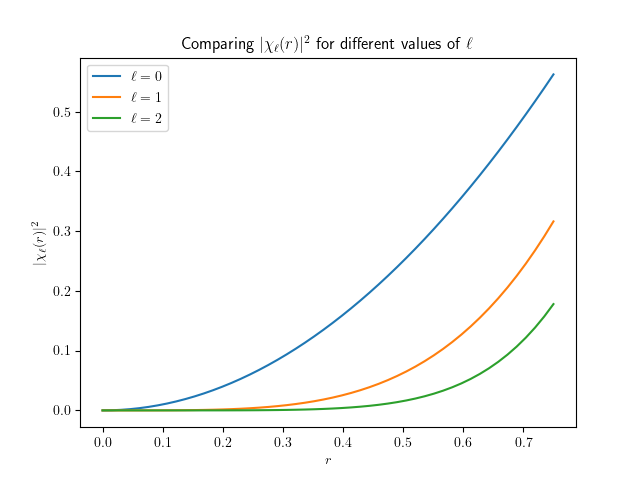
\includegraphics[scale=0.6]{chi_l_squared.png}
    \caption{\(\abs{\chi_\ell(r)}^2\) compared for \(\ell = 0, 1, 2\) and \(r < 1\).}
    \label{fig:chi for low r}
\end{figure}
Figure~\ref{fig:chi for low r} shows \(\abs{\chi_\ell(r)}^2\) plotted for \(\ell = 0, 1, 2\).
We see that the larger the value of \(\ell\) the less likely the particle is to be near the origin.
This can be see as analogous to the classical centrifugal potential which provides a force away from the origin.
In quantum mechanics a centrifugal term in the potential instead decreases the probability of the particle being near the origin.

There are two probabilities that we may be interested in.
The \gls{pdf} for finding the particle at a specific point, \(\vv{r}\) is \(\abs{u(r, \vartheta, \varphi)}^2\) so the probability that the particle is in the volume \(\dd{V}\) is \(\abs{u(r, \vartheta, \varphi)}^2\dd{V}\).
The probability that the particle is in a given volume, \(V\), is then
\[\int_V \abs{u(r, \vartheta, \varphi)}^2.\]
The \gls{pdf} for finding the particle at some specific radius, \(\vv{r}\) is \(\abs{\chi_\ell(r)}^2\) so the probability that the particle is at a point with radius \([r, r + \dd{r}]\) is
\[\int\dd{\Omega}\abs{u(r, \vartheta, \varphi)}^2 = \int\dd{\Omega}\abs{Y_\ell^m(\vartheta, \varphi)}^2\abs{\chi_\ell(r)}^2\dd{r} = \abs{\chi_\ell(r)}^2\dd{r}.\]
The probability that the particle is at some point with a radius in \([a, b]\) is then
\[\int_a^b\dd{r}\abs{\chi_\ell(r)}^2.\]

\section{Spin}
We saw in section~\ref{sec:Bounds on m} that the angular momentum quantum number, \(\ell\), is always an integer despite the fact that the similarly defined \(j\) can take half integer values.
This is because of the spatial dependence of the solutions.
For the eigenfunctions of \(\operator{L}^2\) to be single valued we require that
\[Y_\ell^m(\vartheta, \varphi) = Y_\ell^m(\vartheta, \varphi + 2\pi)\]
and we saw that the \(\varphi\) dependence of \(Y_\ell^m\) was
\[Y_\ell^m(\vartheta, \varphi) \propto e^{im\varphi}.\]
In combination these two equations mean that \(m\) must be an integer.
Since \(m\) takes on any value from \(-\ell\) to \(\ell\) this means that \(\ell\) must be an integer.

\define{Spin} is an intrinsic property of a quantum system.
It is like angular momentum in that the spin is associated with the operator
\[\vecoperator{S} = (\operator{S}_1, \operator{S}_2, \operator{S}_3),\]
with the commutation relation
\[[\operator{S}_k, \operator{S}_l] = i\hbar\varepsilon_{klm}\operator{S}_m.\]
This was the assumption that we made at the start of section~\ref{sec:algebraic solution to the eigenvalue problem} so we can use everything we derived in that section.
In particular we can define 
\[\operator{S}^2 = \operator{S}_x^2 + \operator{S}_y^2 + \operator{S}_z^2.\]
\(\operator{S}^2\) and \(\operator{S}_z\) are a \gls{csco} and have a common eigenbasis:
\[\left\{\ket{s, m}\st m = -s, 1 - s, \dotsc, s - 1, s~\text{and}~s = \frac{n}{2}~\text{where}~n\in\naturals\right\}.\]
The action of \(\operator{S}^2\) and \(\operator{S}_z\) on these basis vectors is
\[\operator{S}^2\ket{s, m} = s(s + 1)\hbar^2\ket{s, m}, \qquad\text{and}\qquad \operator{S}_z\ket{s, m} = m\hbar\ket{s, m}.\]
For a fixed value of \(s\) we see that this is a \((2s + 1)\)-state system.

From now on we focus only on spin 1/2 systems.
That is systems where \(s = 1/2\).
This includes electrons, protons, neutrons, neutrinos, and quarks.
So most matter that we come across day to day.
In this case we have a two dimensional vector space, \(\hilbert_{\text{spin}}\), with a basis
\[\left\{\ket{\tfrac{1}{2}, \tfrac{1}{2}}, \ket{\tfrac{1}{2}, -\tfrac{1}{2}}\right\}.\]
Since \(s = 1/2\) for both of these it is common to introduce a shorter notation where we refer to \(\ket{\tfrac{1}{2}, \tfrac{1}{2}}\) as spin up, denoted \(\ket{\tfrac{1}{2}}\) or \(\ket{\spinUp}\), and \(\ket{\tfrac{1}{2}, -\tfrac{1}{2}}\) as spin down, denoted \(\ket{-\tfrac{1}{2}}\) or \(\ket{\spinDown}\).
These are still eigenfunctions of both \(\operator{S}^2\) and \(\operator{S}_z\):
\[\operator{S}^2\ket{\spinUp} = \frac{3}{4}\hbar^2\ket{\spinUp}, \qquad, \operator{S}^2\ket{\spinDown} = \frac{3}{4}\hbar^2\ket{\spinDown},\]
\[\operator{S}_z\ket{\spinUp} = \frac{\hbar}{2}, \qquad\text{and}\qquad \operator{S}_z\ket{\spinDown} = -\frac{\hbar}{2}\ket{\spinDown}.\]
A generic spin state, \(\ket{\psi}\in\hilbert_\text{spin}\) is given by
\[\ket{\psi} = \psi_1\ket{\spinUp} + \psi_2\ket{\spinDown}\]
where as usual \(\psi_1 = \braket{\spinUp}{\psi}\), \(\psi_2 = \braket{\spinDown}{\psi}\), and \(\abs{\psi_1}^2 + \abs{\psi_2}^2 = 1\).
Since spin has no spatial dependence we describe spin with vectors in \(\hilbert_\text{spin}\).
If a system also has spatial dependence then we can describe this with vectors in some other vector space \(\hilbert_\text{space}\).
The full description of a state is then given by a vector in
\[\hilbert = \hilbert_\text{space}\tensorProd\hilbert_\text{spin}.\]
\(\hilbert\) has as a basis
\[\left\{ \ket{\vv{r}, m}\st \vv{r}\in\reals^3 ~\text{and}~ m = \pm\frac{1}{2} \right\}.\]
The vectors in this basis are simply the tensor products of vectors of the individual bases of \(\hilbert_\text{space}\) and \(\hilbert_\text{spin}\):
\[\ket{\vv{r}, m} = \ket{\vv{r}}\ket{m} = \ket{\vv{r}}\tensorProd\ket{m}.\]
This basis is complete, meaning
\[\int \dd[3]{r'} \sum_{m} \ketbra{\vv{r'}, m}{\vv{r'}, m} = \ident.\]
A generic state, \(\ket{\psi}\in\hilbert\), is then given by
\begin{align*}
    \ket{\psi} &= \int\dd[3]{r} \sum_m \ket{\vv{r'}, m}\braket{\vv{r'}, m}{\psi}\\
    &= \int\dd[3]{r'}\sum_m \psi_m(\vv{r'})\ket{\vv{r'}, m}\\
    &= \int\dd[3]{r'}\left[\psi_1(\vv{r'})\ket{\spinUp} + \psi_2(\vv{r'})\ket{\spinDown}\right]
\end{align*}
where \(\psi_m(\vv{r'}) = \braket{\vv{r'}, m}{\psi}\).
Taking the inner product with a position eigenstate, \(\ket{\vv{r}}\), we have
\begin{align*}
    \braket{\vv{r}}{\psi} &= \int \dd[3]{r'}\sum_m \braket{\vv{r}}{\vv{r'}}\ket{m}\psi_m(\vv{r'})\\
    &= \int \dd[3]{r'} \sum_m \delta(\vv{r} - \vv{r'})\ket{m}\psi_m(\vv{r'})\\
    &= \sum_m \int \dd[3]{r'} \delta(\vv{r} - \vv{r'})\ket{m}\psi_m(\vv{r'})\\
    &= \sum_m \psi_m(\vv{r})\\
    &= \psi_1(\vv{r})\ket{\spinUp} + \psi_2(\vv{r})\ket{\spinDown}.
\end{align*}
In the basis \(\{\ket{\spinUp}, \ket{\spinDown}\}\) for \(\hilbert_\text{spin}\) we can denote \(\braket{\vv{r}}{\psi}\) as a column vector:
\[
\braket{\vv{r}}{\psi} \representation 
\begin{pmatrix}
    \psi_1(\vv{r})\\ \psi_2(\vv{r})
\end{pmatrix}
.
\]
The interpretation of these values is as follows:
\begin{itemize}
    \item \(\abs{\psi_1(\vv{r})^2}\) -- the \gls{pdf} of finding the system at \(\vv{r}\) with spin up.
    \item \(\abs{\psi_2(\vv{r})^2}\) -- the \gls{pdf} of finding the system at \(\vv{r}\) with spin down.
    \item The probability of finding the system anywhere in space with spin up is
    \[P(\spinUp) = \int\dd[3]{r}\abs{\psi_1(\vv{r})}^2.\]
    \item The probability of finding the system anywhere in space with spin down is
    \[P(\spinDown) = \int\dd[3]{r}\abs{\psi_2(\vv{r})}^2.\]
    \item The probability of finding the system at \(\vv{r}\) with any spin is
    \[P(\vv{r}) = \abs{\psi_1(\vv{r})}^2 + \abs{\psi_2(\vv{r})}^2.\] 
\end{itemize}

\subsection{Matrix Elements}
\(\hilbert_{\text{spin}}\) is a two-dimensional vector space.
Therefore the spin operators can be represented by \(2\times 2\) matrices acting on column vectors.
First we start with
\[\operator{S}_z\ket{\spinUp} = \frac{\hbar}{2}\ket{\spinUp}, \qquad\text{and}\qquad \operator{S}_z\ket{\spinDown} = -\frac{\hbar}{2}\ket{\spinDown}.\]
Hence
\begin{align*}
    \bra{\spinUp}\operator{S}_z\ket{\spinUp} &= \frac{\hbar}{2},\\
    \bra{\spinUp}\operator{S}_z\ket{\spinDown} &= 0,\\
    \bra{\spinDown}\operator{S}_z\ket{\spinUp} &= 0,
    \shortintertext{and}
    \bra{\spinDown}\operator{S}_z\ket{\spinDown} &= -\frac{\hbar}{2}.
\end{align*}
This can be written compactly as
\[\bra{m'}\operator{S}_z\ket{m} = \sign(m)\delta_{m'm}\frac{\hbar}{2}.\]
Thus in this basis \(\operator{S}_z\) is represented by
\[
\operator{S}_z \representation \frac{\hbar}{2}
\begin{pmatrix}
    1 & 0\\
    0 & -1
\end{pmatrix}
.
\]
Where we follow the convention that the first row (column) corresponds to the largest value of \(m'\) (\(m\)) so that the first row (column) is labelled by \(m' = 1/2\) (\(m = 1/2\)) and the second row (column) is labelled by \(m' = -1/2\) (\(m = -1/2\)).

As before we define the operators
\[\operator{S}_+ = \operator{S}_x + i\operator{S}_y, \qquad\text{and}\qquad \operator{S}_- = \operator{S}_x - i\operator{S}_y.\]
These have the expected action that
\[\operator{S}_+\ket{\spinUp} = 0, \qquad \operator{S}_+\ket{\spinDown} = \hbar c_+\ket{\spinUp} = \hbar \sqrt{\frac{1}{2}\left(\frac{1}{2} + 1\right) + \frac{1}{2}\left(-\frac{1}{2} + 1\right)}\ket{\spinUp} = \hbar\ket{\spinUp}\]
\[\operator{S}_-\ket{\spinDown} = 0, \qquad\text{and}\qquad \operator{S}_-\ket{\spinUp} = \hbar c_-\ket{\spinDown} = \hbar\sqrt{\frac{1}{2}\left(\frac{1}{2} + 1\right) - \frac{1}{2}\left(\frac{1}{2} + 1\right)} = \hbar\ket{\spinDown}.\]
Hence
\begin{align*}
    \bra{\spinUp}\operator{S}_+\ket{\spinUp} = 0, \qquad & \bra{\spinUp}\operator{S}_-\ket{\spinUp} = 0,\\
    \bra{\spinUp}\operator{S}_+\ket{\spinDown} = \hbar, \qquad & \bra{\spinUp}\operator{S}_-\ket{\spinDown} = 0,\\
    \bra{\spinDown}\operator{S}_+\ket{\spinUp} = 0, \qquad & \bra{\spinDown}\operator{S}_-\ket{\spinUp} = \hbar,\\
    \bra{\spinDown}\operator{S}_+\ket{\spinDown} = 0, \qquad & \bra{\spinDown}\operator{S}_-\ket{\spinDown} = 0.
\end{align*}
Thus in this basis these operators are represented by
\[
\operator{S}_+ \representation\hbar
\begin{pmatrix}
    0 & 1\\
    0 & 0
\end{pmatrix}
\qquad\text{and}\qquad
\operator{S}_- \representation\hbar
\begin{pmatrix}
    0 & 0\\
    1 & 0
\end{pmatrix}
.
\]
Now we can write
\[\operator{S}_x = \frac{1}{2}\left(\operator{S}_+ + \operator{S_-}\right), \qquad\text{and}\qquad \operator{S}_y = \frac{1}{2i}\left(\operator{S}_+ - \operator{S}_-\right).\]
Thus the representations of \(\operator{S}_x\) and \(\operator{S}_y\) in this basis are
\[
\operator{S}_x \representation \frac{\hbar}{2}
\begin{pmatrix}
    0 & 1\\
    1 & 0
\end{pmatrix}
\qquad\text{and}\qquad
\operator{S}_y \representation \frac{\hbar}{2}
\begin{pmatrix}
    0 & -i\\
    i & 0
\end{pmatrix}
.
\]
The three matrices representing \(\operator{S}_k\) in this basis are called the \define{Pauli spin matrices}:
\[
\sigma_x =
\begin{pmatrix}
    0 & 1\\
    1 & 0
\end{pmatrix}
,\qquad \sigma_y =
\begin{pmatrix}
    0 & -i\\
    i & 0
\end{pmatrix}
,\qquad\text{and}\qquad \sigma_z = 
\begin{pmatrix}
    1 & 0\\
    0 & 1
\end{pmatrix}
.
\]
Which allows us to compactly write
\[\operator{S}_k \representation \frac{\hbar}{2}\sigma_k, \qquad\text{and}\qquad \vecoperator{S} = \frac{\hbar}{2}\vv{\sigma}\]
where \(\vv{\sigma} = (\sigma_x, \sigma_y, \sigma_z)\).
The Pauli matrices are Hermitian, as they are associated with observables, and also unitary, meaning \(\sigma_k\sigma_k\hermit = \sigma_k^2 = \ident\), they also all have zero trace, \(\tr(\sigma_k) = 0\).
We can then use \(\sigma\) as another label for the basis vectors, for example if we define
\[\ket{\psi} = \sum_{\sigma} \psi_\sigma\ket{\sigma}\]
then we can characterise the action of \(\operator{S}_k\) as
\[\ket{\varphi} = \operator{S}_k = \sum_\sigma \varphi_\sigma\ket{\sigma} = \sum_\sigma\sum_{\sigma'}(S_k)_{\sigma\sigma'}\psi_{\sigma'}\ket{\sigma}\]
where we have used
\[\varphi_\sigma = \sum_{\sigma'}(S_k)_{\sigma\sigma'}\psi_{\sigma'}.\]

We can now use the definition of \(\operator{S}^2\) to find a representation for \(\operator{S}^2\) in this basis:
\begin{align*}
    \operator{S}^2 &= \sum_k \operator{S}_k^2\\
    &\representation \sum_k \left(\frac{\hbar}{2}\sigma_k\right)^2\\
    &= \sum_k \frac{\hbar^2}{4}\sigma_k^2\\
    &= \sum_k \frac{\hbar^2}{4}\ident\\
    &= \frac{3}{4}\hbar^2\ident\\
    &= \frac{3}{4}\hbar^2
    \begin{pmatrix}
        1 & 0\\
        0 & 1
    \end{pmatrix}
\end{align*}

\subsection{Eigenvectors of \texorpdfstring{\(\operator{S}_z\)}{Sz} and \texorpdfstring{\(\operator{S}^2\)}{S2}}
The eigenvectors of \(\sigma_z\) are easy to find:
\[
\begin{pmatrix}
    1 & 0\\
    0 & -1
\end{pmatrix}
\begin{pmatrix}
    1\\ 0
\end{pmatrix}
=
\begin{pmatrix}
    1\\ 0
\end{pmatrix}
,\qquad\text{and}\qquad
\begin{pmatrix}
    1 & 0\\
    0 & -1
\end{pmatrix}
\begin{pmatrix}
    0\\ 1
\end{pmatrix}
= -
\begin{pmatrix}
    0\\ 1
\end{pmatrix}
.
\]
So the eigenvalues of this representation of \(\operator{S}_z\) are given by
\[
\frac{\hbar}{2}
\begin{pmatrix}
    1 & 0\\
    0 & -1
\end{pmatrix}
\begin{pmatrix}
    1\\ 0
\end{pmatrix}
= \frac{\hbar}{2}
\begin{pmatrix}
    1\\ 0
\end{pmatrix}
,\qquad\text{and}\qquad
\frac{\hbar}{2}
\begin{pmatrix}
    1 & 0\\
    0 & -1
\end{pmatrix}
\begin{pmatrix}
    0\\ 1
\end{pmatrix}
= -\frac{\hbar}{2}
\begin{pmatrix}
    0\\ 1
\end{pmatrix}
.
\]
We see that these have the eigenvalues \(\pm\hbar/2\), which is what we would expect for a spin 1/2 system.
These eigenvectors are also simultaneously eigenvectors of \(\operator{S}^2\) in this representation, this is trivial since \(\operator{S}^2\) is proportional to the identity in this representation:
\[
\frac{3}{4}\hbar^2
\begin{pmatrix}
    1 & 0\\
    0 & 1
\end{pmatrix}
\begin{pmatrix}
    1\\ 0
\end{pmatrix}
= \frac{3}{4}\hbar^2
\begin{pmatrix}
    1\\ 0
\end{pmatrix}
,\qquad\text{and}\qquad
\frac{3}{4}\hbar^2
\begin{pmatrix}
    1 & 0\\
    0 & 1
\end{pmatrix}
\begin{pmatrix}
    0\\ 1
\end{pmatrix}
= \frac{3}{4}\hbar^2
\begin{pmatrix}
    0\\ 1
\end{pmatrix}
.
\]
Thus we can identify
\[
\ket{s=\tfrac{1}{2}, m=\tfrac{1}{2}} = \ket{\spinUp} \representation 
\begin{pmatrix}
    0\\ 1
\end{pmatrix}
,\qquad\text{and}\qquad
\ket{s = \tfrac{1}{2}, m=-\tfrac{1}{2}} = \ket{\spinDown} \representation
\begin{pmatrix}
    1\\ 0
\end{pmatrix}
.
\]
A generic vector, \(\ket{\psi}\in\hilbert_{\text{spin}}\), can then be represented by
\[
\ket{\psi} = \psi_1\ket{\spinUp} + \psi_2\ket{\spinDown} \representation
\begin{pmatrix}
    \psi_1\\
    \psi_2
\end{pmatrix}
=
\psi_1
\begin{pmatrix}
    1\\ 0
\end{pmatrix}
+ \psi_2
\begin{pmatrix}
    0\\ 1
\end{pmatrix}
.
\]
Note that in general \(\psi_k\in\complex\) so the space spanned by these eigenvectors is not \(\reals^2\) but \(\complex^2\).

\subsection{Scalar Products}
Now that we have representations of generic vectors in this basis we ask what is the representation of a covector, \(\bra{\psi}\in\hilbert_{\text{spin}}^*\)?
The answer, as always, is that if \(\ket{\psi}\) is represented by an \(n\)-dimensional column vector then \(\bra{\psi}\) is represented by an \(n\)-dimensional row vector with the components given by
\[
\ket{\psi} \representation 
\begin{pmatrix}
    \psi_1\\ \psi_2
\end{pmatrix}
\implies
\bra{\psi} \representation
\begin{pmatrix}
    \psi_1^* & \psi_2^*
\end{pmatrix}
.
\]
That is \(\bra{\psi} = (\ket{\psi})\hermit\).
The scalar product of two states, \(\ket{\psi}\) and \(\ket{\varphi}\), is then
\[
\braket{\varphi}{\psi} =
\begin{pmatrix}
    \varphi_1^* & \varphi_2^*
\end{pmatrix}
\begin{pmatrix}
    \psi_1\\ \psi_2
\end{pmatrix}
= \varphi_1^*\psi_1 + \varphi_2^*\psi_2.
\]
For example if \(\ket{\psi}\) is a properly normalised state then
\[
\braket{\varphi}{\psi} =
\begin{pmatrix}
    \psi_1^* & \psi_2^*
\end{pmatrix}
\begin{pmatrix}
    \psi_1\\ \psi_2
\end{pmatrix}
= \abs{\psi_1}^2 + \abs{\varphi_2}^2  = 1.
\]

\subsection{Spin Along the \texorpdfstring{\(x\)}{x} Direction}
We can find the possible values of \(m_x\) by finding the eigenvalues of \(\hbar\sigma_x/2\) in the \(\operator{S}_z\) eigenbasis.
We do this in the normal way:
\begin{align*}
    0 &= \det\left(\frac{\hbar}{2}\sigma_x - \lambda\ident\right)\\
    &= 
    \begin{vmatrix}
        -\lambda & \hbar/2\\
        \hbar/2 & -\lambda
    \end{vmatrix}
    \\
    &= \lambda^2 - \frac{\hbar^2}{4}
\end{align*}
So \(S_x = \lambda = \pm \hbar/2\).
This is the same as the possible values of \(S_z\), this is what we would expect from the symmetry of the situation, there is nothing important about the \(z\) or \(x\) directions that would mean they have different possible values of \(S_k\).
We can write a state with \(m_x = 1/2\) as a combination of the basis vectors:
\[\ket{m_x = 1/2} = \alpha\ket{\spinUp} + \beta\ket{\spinDown}.\]
In this representation this becomes
\[
\operator{S}_x\ket{m_x = 1/2} = \frac{\hbar}{2}\ket{m_x = 1/2} \representation \frac{\hbar}{2}\sigma_x
\begin{pmatrix}
    \alpha\\ \beta
\end{pmatrix}
=
\frac{\hbar}{2}
\begin{pmatrix}
    0 & 1\\
    1 & 0
\end{pmatrix}
\begin{pmatrix}
    \alpha\\ \beta
\end{pmatrix}
= \frac{\hbar}{2}
\begin{pmatrix}
    \beta\\ \alpha
\end{pmatrix}
= \frac{\hbar}{2}
\begin{pmatrix}
    \alpha\\ \beta
\end{pmatrix}
.
\]
Hence \(\alpha = \beta\) so a properly normalised state with \(m_x = \hbar/2\) is
\[\ket{m_x = 1/2} = \frac{\sqrt{2}}{2}\left[\ket{\spinUp} + \ket{\spinDown}\right].\]
We can show in a similar way that if \(S_x = -1/2\) then
\[\ket{m_x = -1/2} = \frac{\sqrt{2}}{2}\left[\ket{\spinUp} - \ket{\spinDown}\right].\]

It can be shown that if we measure the spin along any vector in the \((x, z)\)-plane at an angle \(\vartheta\) to the \(z\) axis,
\[\vh{n} = \sin(\vartheta)\ve{x} + \cos(\vartheta)\ve{z},\]
then the relevant eigenstates in the the representation that we are using are the eigenvalues of
\[
\vv{\sigma}\cdot\vh{n} = \sigma_x\sin(\vartheta) + \sigma_z\cos(\vartheta) = 
\begin{pmatrix}
    \cos\vartheta & \sin\vartheta\\
    \sin\vartheta & -\cos\vartheta
\end{pmatrix}
.
\]

\section{Addition of Angular Momenta}\label{sec:addition of angular momenta}
Suppose we have two systems with independent angular momenta \(\vecoperator{J}^{(1)}\) and \(\vecoperator{J}^{(2)}\).
This could be two particles with angular momentum, two particles with spin or one particle with angular momentum and spin.
These operators satisfy the usual commutation relations,
\[\left[\operator{J}^{(n)}_k, \operator{J}^{(n)}_l\right] = i\hbar\varepsilon_{klm}\operator{J}^{(n)}_m, \qquad\text{and}\qquad \left[\angmomsquared{n}, \operator{J}^{(n)}_k\right] = 0.\]
Since the two angular momenta are independent the operators associated with different angular momenta commute:
\[\left[\operator{J}^{(1)}_k, \operator{J}^{(2)}_l\right] = \left[\angmomsquared{1}, \angmomsquared{2}\right] = \left[\angmomsquared{1}, \operator{J}^{(2)}_k\right] = 0 \qquad\text{etc.}\]
We can extend this easily to any number of independent angular momenta but we won't here.

\subsection{Vector Spaces}
Since \(\vecoperator{J}^{(1)}\) and \(\vecoperator{J}^{(2)}\) commute they form a \gls{csco} which means we can find a common eigenbasis.
Since both angular momenta are independent we can describe both with separate Hilbert spaces.
Angular momentum 1 is described by vectors in a vector space \(\hilbert^{(1)}\).
For a particular value, \(j^{(1)}\), of the angular momentum quantum number this is a \(2j_1 + 1\) dimensional vector space.
This space has as a basis \(\{\ket{j_1, m_1}\}\)
Similarly angular momentum 2 is described by vectors in the \(2j_2 + 1\) dimensional vector space, \(\hilbert^{(2)}\), with basis \(\ket{j_2, m_2}\).
The entire system is then described by vectors in
\[\hilbert = \hilbert^{(1)}\tensorProd\hilbert^{(2)}.\]
The dimensionality of this vector space is
\[\dim(\hilbert) = \dim(\hilbert^{(1)})\dim(\hilbert^{(2)}) = (2j_1 + 1)(2j_2 + 1).\]
This space then has as a basis
\[\{\ket{j_1, m_1, j_2, m_2}\} = \{\ket{j_1, m_1}\tensorProd\ket{j_2, m_2}\}.\]
As usual we extend the definition of the operators so that they act on only their respective parts of these vectors.
Strictly we should define new operators like \({\operator{J}^{(1)}_z}{'} = \operator{J}^{(1)}_z\tensorProd\ident\) which then acts on \(\ket{j_1, m_1, j_2, m_2} = \ket{j_1, m_1}\tensorProd\ket{j_2, m_2}\) as
\begin{align*}
    {\operator{J}^{(1)}_z}{'}\ket{j_1, m_1, j_2, m_2} &= (\operator{J}^{(1)}_z\tensorProd\ident)(\ket{j_1, m_1}\tensorProd\ket{j_2, m_2})\\
    &= \operator{J}^{(1)}_z\ket{j_1, m_1}\tensorProd\ident\ket{j_2, m_2}\\
    &= \hbar m_1\ket{j_1, m_1}\tensorProd\ket{j_2, m_2}\\
    &= \hbar m_1\ket{j_1, m_1, j_2, m_2}
\end{align*}
but in practice we use the same symbol for both operators, \(\operator{J}^{(1)}_z\colon\hilbert^{(1)}\to\complex\) and \(\operator{J}^{(1)}_z{'}\colon\hilbert\to\complex\).
The action of the operators on this basis is
\begin{align*}
    \angmomsquared{1}\ket{j_1, m_1, j_2, m_2} &= \hbar^2j_1(j_1 + 1)\ket{j_1, m_1, j_2, m_2},\\
    \operator{J}^{(1)}_z\ket{j_1, m_1, j_2, m_2} &= \hbar m_1\ket{j_1, m_1, j_2, m_2},\\
    \angmomsquared{2}\ket{j_1, m_1, j_2, m_2} &= \hbar^2j_2(j_2 + 1)\ket{j_1, m_1, j_2, m_2},\\
    \operator{J}^{(2)}_z\ket{j_1, m_1, j_2, m_2} &= \hbar m_2\ket{j_1, m_1, j_2, m_2}.
\end{align*}
A generic state, \(\ket{\psi}\in\hilbert\), can be given as
\[\ket{\psi} = \sum_{j_1, m_2, j_2, m_2} c_{j_1m_1j_2m_2}\ket{j_1, m_1, j_2, m_2}\]
where
\[c_{j_1m_1j_2m_2} = \braket{j_1, m_1, j_2, m_2}{\psi}.\]

\subsection{Total Angular Momentum}\label{sec:total angular momentum}
We can now define the total angular momentum:
\[\vecoperator{J} = \vecoperator{J}^{(1)} + \vecoperator{J}^{(2)}.\]
This satisfies the normal angular momentum commutation relations:
\[[\operator{J}_k, \operator{J}_l] = i\hbar\varepsilon_{klm}\operator{J}_m, \qquad\text{and}\qquad [\operator{J}^2, \operator{J}_k] = 0.\]
This means that \(\operator{J}^2\) and \(\operator{J}_z\) form a \gls{csco} so we can find a simultaneous eigenbasis for \(\hilbert\) made of vectors of the form \(\{\ket{j, m}\}\).
What values can \(j\) and \(m\) take?
The answer lies in the angular momentum addition theorem, which we won't prove here:
\begin{theorem}{Angular momentum addition theorem}{}
    Given two independent angular momenta with corresponding quantum numbers, \(j_1\) and \(j_2\), the allowed value of the angular momentum quantum number for the total angular momentum are
    \[j = j_1 + j_2, j_1 + j_2 - 1, \dotsc, \abs{j_1 - j_2}.\]
    For each of these values we also have
    \[m = -j, -j + 1, \dotsc, j - 1, j.\]
\end{theorem}
Before we said that \(\dim(\hilbert) = (2j_1 + 1)(2j_2 + 1)\).
We can check that this is consistent with the angular momentum addition theorem.
Without loss of generality assume that \(j_1 \ge j_2\).
Then
\begin{align*}
    \dim(\hilbert) &= \sum_{\mathclap{j=j_1 - j_2}}^{\mathclap{j_1 + j_2}} (2j + 1)\\
    &= \sum_{j=0}^{\mathclap{j_1 + j_2}} (2j + 1) - \sum_{j = 0}^{\mathclap{j_1 - j_2 - 1}} (2j + 1)\\
    &= 2\sum_{j=0}^{\mathclap{j_1 + j_2}} j + (j_1 + j_2) - 2\sum_{j = 0}^{\mathclap{j_1 - j_2 - 1}} j - (j_1 - j_2 - 1 )\\
    &= (j_1 + j_2)(j_1 + j_2 + 1) + (j_1 + j_2) - (j_1 - j_2 - 1)(j_1 - j_2) - (j_1 - j_2 - 1)\\
    &= j_1^2 + j_2^2 + 2j_1j_2 + j_1 + j_2 + j_1 + j_2 - j_1^2 - j_2^2 + 2j_1j_2 + j_1 - j_2 - j_1 + j_2 + 1\\
    &= 4j_1j_2 + 2j_1 + 2j_2 + 1\\
    &= (2j_1 + 1)(2j_2 + 1).\\
\end{align*}
Where we have used
\[\sum_{r = 0}^n = \frac{1}{2}n(n + 1),\]
which is proven in appendix~\ref{sec:proof sum 0 to n of r is 0.5 n(n+1)}.
Both bases, \(\{\ket{j_1, m_1, j_2, m_2}\}\) and \(\{\ket{j, m}\}\), are orthonormal so there exists a unitary transformation between the two bases.
For fixed \(j_1\) and \(j_2\) we denote \(\ket{j, m}\) as \(\ket{j, m; j_1, j_2}\) to denote the specific values that \(j_1\) and \(j_2\) are held at.
Using the completeness of the \(\{\ket{j_1, m_1, j_2, m_2}\}\) basis,
\[\sum_{m_1, m_2} \braket{j_1, m_1, j_2, m_2}{j_1, m_1, j_2, m_2} = \ident\]
we have
\[\ket{j, m; j_1, j_2} = \sum_{m_1, m_2} \ket{j_1, m_1, j_2, m_2}\braket{j_1, m_1, j_2, m_2}{j, m; j_1, j_2}.\]
The quantities \(\braket{j_1, m_1, j_2, m_2}{j, m; j_1, j_2}\) are called the Clebsch--Gordan coefficients and they are tabulated in many sources.

The basis \(\{\ket{j_1, m_1, j_2, m_2}\}\) is called the \define{uncoupled basis} as vectors in this basis can be written as two parts, one related to angular momentum 1 and the other related to angular momentum 2, for example a basis vector can be written as \(\ket{j_1, m_1}\tensorProd\ket{j_2, m_2}\) and a generic vector as
\[\ket{\psi} = \sum_{\mathclap{j_1, m_1, j_2, m_2}}(\braket{j_1, m_1}{\psi}\ket{j_1, m_1} \tensorProd\braket{j_2, m_2}{\psi}\ket{j_2, m_2}).\]
The basis \(\{\ket{j, m}\}\) is called the \define{coupled basis} as this is not possible.

\begin{example}
    Consider a system composed of two spin 1/2 particles.
    \(\hilbert^{(1)}\) is a two dimensional vector space with a basis
    \[\{s_1, m_1\} = \{\ket{\tfrac{1}{2}, \tfrac{1}{2}}, \ket{\tfrac{1}{2}, -\tfrac{1}{2}}\}.\]
    \(\hilbert^{(2)}\) is also a two dimensional vector space with basis
    \[\{s_2, m_2\} = \{\ket{\tfrac{1}{2}, \tfrac{1}{2}}, \ket{\tfrac{1}{2}, -\tfrac{1}{2}}\}.\]
    The spin of the whole system is then characterised by vectors in \(\hilbert = \hilbert^{(1)}\tensorProd\hilbert^{(2)}\) which has the basis
    \[\{\ket{s_1, m_1, s_2, m_2}\} = \{\ket{\tfrac{1}{2},\tfrac{1}{2},\tfrac{1}{2},\tfrac{1}{2}}, \ket{\tfrac{1}{2},\tfrac{1}{2},\tfrac{1}{2},-\tfrac{1}{2}}, \ket{\tfrac{1}{2},-\tfrac{1}{2},\tfrac{1}{2},\tfrac{1}{2}}, \ket{\tfrac{1}{2},-\tfrac{1}{2},\tfrac{1}{2},-\tfrac{1}{2}}\}.\]
    Since \(s_i = 1/2\) for all states in this system we compactly write this basis as
    \[\{\ket{\spinUp\spinUp}, \ket{\spinUp\spinDown}, \ket{\spinDown\spinUp}, \ket{\spinDown, \spinDown}\}.\]
    Where the first arrow denotes particle 1's spin and the second arrow denotes particle 2's spin.
    The values that \(s\) can take, as given by the angular momentum addition theorem, is \(s = s_1 + s_2, \abs{s_1 - s_2} = 1, 0\).
    So the entire system has spin 1 or spin 0.
    To find the uncoupled basis consider the action of \(\operator{S}_z\) on the coupled basis
    \[\operator{S}_z\ket{\spinUp\spinUp} = (\operator{S}^{(1)}_z + \operator{S}^{(2)}_z)\ket{\spinUp\spinUp} = \frac{\hbar}{2}\ket{\spinUp\spinUp} + \frac{\hbar}{2}\ket{\spinUp\spinUp} = \hbar\ket{\spinUp\spinUp}.\]
    Hence \(m = 1\).
    Since \(m > 0\) we know that \(s \ne 0\) so \(s = 1\).
    Similarly
    \[\operator{S}_z\ket{\spinDown\spinDown} = (\operator{S}^{(1)}_z + \operator{S}^{(2)}_z)\ket{\spinDown\spinDown} = -\frac{\hbar}{2}\ket{\spinDown\spinDown} + -\frac{\hbar}{2}\ket{\spinDown\spinDown} = -\hbar\ket{\spinDown\spinDown}.\]
    Hence \(m = 1\) and \(s = 1\) for this state.
    So far we have
    \[\ket{1,1} = \ket{\spinUp\spinUp}, \qquad\text{and}\qquad \ket{1,-1} = \ket{\spinDown\spinDown}.\]
    We don't yet know what \(\ket{1, 0}\) or \(\ket{0, 0}\) are.
    The difficulty in finding these states is that they aren't uniquely identified purely by the value of \(m\).
    However we do know how to construct them from other states using raising and lowering operators.
    The lowering operator for the total angular momentum is simply
    \[\operator{S}_- = \operator{S}^{(1)}_- + \operator{S}^{(2)}_-\]
    so by identifying that we expect
    \[\operator{S}_-\ket{1, 1} \propto \ket{1, 0}\]
    we know that
    \[\ket{1, 0} \propto \operator{S}_-\ket{\spinUp\spinUp} = (\operator{S}^{(1)}_- + \operator{S}^{(2)}_-)\ket{\spinUp\spinUp} = \operator{S}^{(1)}_-\ket{\spinUp\spinUp} + \operator{S}^{(2)}_-\ket{\spinUp\spinUp} \propto \ket{\spinDown\spinUp} + \ket{\spinUp\spinDown}.\]
    Using the fact that the uncoupled basis vectors are orthonormal we have
    \[\ket{1, 0} = \frac{\sqrt{2}}{2}(\ket{\spinUp\spinDown} + \ket{\spinUp\spinDown}).\]
    Finally \(\ket{0, 0}\) must be a linear combination of \(\ket{\spinUp\spinDown}\) and \(\ket{\spinDown\spinUp}\) and it must be orthogonal to \(\ket{1, 0}\).
    We are then free to chose that
    \[\ket{0, 0} = \frac{\sqrt{2}}{2}(\ket{\spinUp\spinDown} - \ket{\spinDown\spinUp}).\]
    This agrees with the Clebsch--Gordan coefficients which are tabulated in table~\ref{tab:clebsch-gordan coefficients j = 1}.
    \begin{table}[ht]
        \centering
        \begin{subtable}{0.25\textwidth}
            \centering
            \begin{tabular}{|l|l|}\hline
                \backslashbox{\(m_1, m_2\)}{\(j\)} & 1\\ \hline
                \(1/2, 1/2\) & 1\\ \hline
            \end{tabular}
            \subcaption{\(m = 1\)}
        \end{subtable}
        \begin{subtable}{0.25\textwidth}
            \centering
            \begin{tabular}{|l|l|}\hline
                \backslashbox{\(m_1, m_2\)}{\(j\)} & 1\\ \hline
                \(-1/2, -1/2\) & 1\\ \hline
            \end{tabular}
            \subcaption{\(m = -1\)}
        \end{subtable}
        \begin{subtable}{0.4\textwidth}
            \centering
            \begin{tabular}{|l|l|l|}\hline
                \backslashbox{\(m_1, m_2\)}{\(j\)} & 1 & 0\\ \hline
                \(1/2, -1/2\) & \(\sqrt{2}/2\) & \(\sqrt{2}/2\)\\ \hline
                \(-1/2, 1/2\) & \(\sqrt{2}/2\) & -\(\sqrt{2}/2\)\\ \hline
            \end{tabular}
            \subcaption{\(m = 0\)}
        \end{subtable}
        
        
        \caption{Clebsch--Gordan coefficients for two spin 1/2 particles.}
        \label{tab:clebsch-gordan coefficients j = 1}
    \end{table}
\end{example}

\section{Identical Particles}
In classical mechanics if we have two particles that have all the same properties, like mass, charge, angular momentum, etc. then we can still tell them apart from the fact that one of them is `here' and the other is `there'.
Even at some later time we can still tell them apart as we can track their trajectories back to a time when we could tell them apart.
In \gls{qm} this is not possible.
If two particles have the same properties, meaning identical quantum numbers, \(n\), \(\ell\), \(s\), \(m\), etc. then we label one `particle 1' and the other `particle 2' we lose this information as soon as we ascribe it as the system evolves and since there is no concept of trajectory we can't tell which particle was which at some earlier time.

To think about this mathematically we start with the states, \(\ket{\xi_1}, \ket{\xi_2}\in\hilbert\), which describe each particle.
The two particle system is then described by \(\ket{\xi_1, \xi_2} = \ket{\xi_1}\tensorProd\ket{\xi_2} \in\hilbert \tensorProd\hilbert\).

Here particle 1 and 2 are labels that we assign that distinguish the particles for the sake of the maths.
There is no way to look at a particle and tell if it is particle 1 or 2.
We define an operator, \(\operator{\parity}_{12}\) which swaps particle 1 and 2.
That is
\[\operator{\parity}_{12}\ket{\xi_1, \xi_2} = \ket{\xi_2, \xi_1}.\]
Since quantum states are defined up to a phase factor and swapping the two particles doesn't change the state of the system we must have that
\[\ket{\xi_1, \xi_2} = e^{i\alpha}\ket{\xi_2, \xi_1}\]
for some \(\alpha\in\reals\).
By swapping the two states again we get back to the original state and we pick up another phase factor:
\[\ket{\xi_1, \xi_2} = e^{2i\alpha}\ket{\xi_1, \xi_2}.\]
This can only be true if \(e^{2i\alpha} = 1\) which means that \(e^{i\alpha} = \pm 1\), thus \(\alpha = n\pi\) for \(n\in\integers\).
This means that this state is either symmetric or antisymmetric under swapping the particles.
It turns out that there is a theorem that allows us to be even more precise than this, which we will not prove here.
It is called the spin statistics theorem:
\begin{theorem}{Spin Statistics Theorem}{}
    Particles with integer spin, \(s = 0, 1, 2, \dotsc\), are symmetric under swapping identical particles:
    \[\ket{\xi_1, \xi_2} = \ket{\xi_2, \xi_1}.\]
    Such particles are called \define{bosons} and are described by Bose--Einstein statistics.
    
    Particles with half integer spin, \(s = 1/2, 3/2, 5/2, \dotsc\), are antisymmetric under swapping identical particles:
    \[\ket{\xi_1, \xi_2} = - \ket{\xi_2, \xi_1}.\]
    Such particles are called \define{fermions} and are described by Fermi--Dirac statistics.
\end{theorem}

\subsection{Helium Atom}
A helium atom, \ce{He}, has two electrons.
These electrons are identical particles.
There is also a proton.
The interaction of one electron and the proton has a Hamiltonian given by
\[\operator{H}_i = \frac{\vecoperator{P}\cdot\vecoperator{P}}{2\mu} - \frac{2e^2}{r_i}\]
where \(i = 1, 2\) denotes the particle number, \(\mu\) is the mass of the electron, \(e\) is the magnitude of the charge of the electron and proton, and \(r_i\) denotes the distance of electron \(i\) from the proton.
The entire system can then be described as the Hamiltonian for each electron plus a term characterising the interaction of the two electrons:
\[\operator{H} = \operator{H}_1 + \operator{H}_2 + \frac{e^2}{\abs{\vv{r_1} - \vv{r_2}}}.\]
Notice that \(\operator{H}\) is symmetric under \(\operator{\parity}_{12}\).
That is \(\operator{H}(1, 2) = \operator{H}(2, 1)\) where \(\operator{H}(1, 2)\) is \(\operator{H}\) as defined above and \(\operator{H}(2, 1) = \operator{\parity}_{12}\operator{H}(1, 2)\).
The \gls{tise} for this system is
\[\operator{H}(1, 2)\ket{\xi_1, \xi_2} = E\ket{\xi_1, \xi_2},\]
where we now require that \(\ket{\xi_1, \xi_2}\) is an energy eigenstate.
We now rename 1 to 2 and 2 to 1, this changes nothing other than labels:
\[\operator{H}(2, 1)\ket{\xi_2, \xi_1} = E\ket{\xi_2, \xi_1}.\]
Finally using the fact that \(\operator{H}(1, 2) = \operator{H}(2, 1)\) we have that
\[\operator{H}(1, 2)\ket{\xi_2, \xi_2} = E\ket{\xi_2, \xi_2}.\]
Thus any given eigenstate, \(\ket{\xi_1, \xi_2}\), of \(\operator{H}(1, 2)\), gives us another eigenstate, \(\ket{\xi_2, \xi_1}\).
We can define a symmetric and antisymmetric state, \(\ket{+}\) and \(\ket{-}\) respectively, in the usual way:
\[\ket{\psi\pm} = \frac{\sqrt{2}}{2}(\ket{\xi_1, \xi_2} \pm \ket{\xi_2, \xi_1}).\]
The action of \(\operator{\parity}_{12}\) on these is
\[\operator{\parity}_{12}\ket{\pm} = \pm\ket{\pm}.\]
So \(\ket{\pm}\) are eigenstates of \(\operator{\parity}_{12}\), with eigenvalues \(\pm 1\) and \(\operator{H}\), with eigenvalues \(E\).
Hence \([\operator{H}, \operator{\parity}_{12}] = 0\).
This means that the symmetry properties of the system are preserved in time since this means that \(\operator{\parity}_{12}\) commutes with the time evolution operator.

\subsection{Two Electron State}
Consider now a system made of two electrons.
There are sets of degrees of freedom to consider.
The spatial degrees of freedom, described by vectors in \(\hilbert_{\text{space}}\), and the spin degrees of freedom, described by vectors in \(\hilbert_{\text{spin}}\).
Both electrons have \(s_i = 1/2\) so by the angular momenta addition theorem the total spin of the system is \(s = 0, 1\).
In the case where \(s = 0\) we must also have \(m = 0\) so \(\ket{0, 0}\) is the only state with \(s = 0\), we call this a singlet state.
In the case where \(s = 1\) we have \(m = -1, 0, 1\) so there are three states, \(\ket{1, -1}\), \(\ket{1, 0}\), and \(\ket{1, 1}\), with \(s = 1\), we call this a triplet state.
We have previously shown that in the uncoupled basis these states are
\[\ket{0, 0} = \frac{\sqrt{2}}{2}(\ket{\spinUp\spinDown} - \ket{\spinDown\spinUp}), \qquad \ket{1, 1} = \ket{\spinUp\spinUp}, \qquad \ket{1, -1} = \ket{\spinDown\spinDown}, \qquad\text{and}\qquad \ket{1, 0} = \frac{\sqrt{2}}{2}(\ket{\spinUp\spinDown} + \ket{\spinDown\spinUp}).\]
From this we can see that \(\ket{0, 0}\) is antisymmetric under swapping of the two particles and all the other states are symmetric.
Let \(\ket{\psi_{12}}\hilbert_{\text{space}}\) be a generic state describing the spatial degrees of freedom.
The a generic state, \(\ket{\Psi} \in \hilbert = \hilbert_{\text{space}}\tensorProd\hilbert_{\text{spin}}\) with \(s = 1\) is given by
\[\ket{\Psi} = \ket{\psi_{12}}\tensorProd\ket{s=1, m}.\]
Using the fact that \(s = 1\) implies that \(\ket{s=1, m}\) is symmetric under \(\operator{\parity}_{12}\) the action of swapping the two particles is given by
\begin{align*}
    \operator{\parity}_{12}\ket{\Psi} &= (\operator{\parity}_{12}\ket{\psi_{12}}) \tensorProd (\operator{\parity}_{12}\ket{s=1, m})\\
    &= (\operator{\parity}_{12}\ket{\psi_{12}}) \tensorProd \ket{s=1, m}\\
    &= -\ket{\Psi}.
\end{align*}
Here we have used that electrons are spin 1/2 particles so by the spin statistics theorem the overall state describing them is antisymmetric.
The only way to have this be true is to have \(\ket{\psi_{12}}\) be antisymmetric under \(\operator{\parity_{12}}\).
Similarly a generic state with \(s=0\) is described by
\[\ket{\Psi} = \ket{\psi_{12}}\tensorProd\ket{s=0, m=0}.\]
Again this is antisymmetric under \(\operator{\parity_{12}}\) but this time \(\ket{s=0, m=0}\) is antisymmetric under \(\operator{\parity_{12}}\) so \(\ket{\psi_{12}}\) must be symmetric under \(\operator{\parity_{12}}\).
These two results are tabulated in table~\ref{tab:symmetry under swapping of particles}.
\begin{table}[ht]
    \centering
    \begin{tabular}{cccc}\hline
        \(s\) & \(\ket{s, m}\) & \(\ket{\psi_{12}}\) & \(\ket{\Psi}\)\\\hline
        0 & A & S & A\\
        1 & S & A & A\\\hline
    \end{tabular}
    \caption{The symmetry of various parts of a state under \(\operator{\parity_{12}}\). S denotes symmetric and A denotes antisymmetric. The symmetry of the total system, \(\ket{\Psi}\), is set by the spin statistics theorem. The symmetry of the spin part, \(\ket{s, m}\), follows from the expression in the uncoupled basis. The symmetry of the spatial part, \(\ket{\psi_{12}}\), is then fixed to make the symmetries of the other parts match.}
    \label{tab:symmetry under swapping of particles}
\end{table}
\subsection{Pauli Exclusion Principle}
One consequence of the spin statistics theorem is the \define{Pauli exclusion principle}, that no two fermions can be in the same state.
The reason for this is that if particles 1 and 2 are identical fermions and \(\ket{\xi_1} = \ket{\xi_2}\) then by the spin statistics theorem
\[\ket{\xi_1, \xi_2} = -\ket{\xi_2, \xi_1} = -\ket{\xi_1, \xi_2}\]
where for the first equality we use the spin statistics theorem and for the second the fact that \(\ket{\xi_1} = \ket{\xi_2}\).
The only solution to this equation is \(\ket{\xi_1, \xi_2} = 0\) but this is not a valid state, it isn't normalisable for one.
Therefore we cannot have \(\ket{\xi_1} = \ket{\xi_2}\) if the spin statistics theorem holds.

\section{The Hydrogen Atom}
In this section we will give a non-relativistic treatment of the hydrogen atom.
We model the hydrogen atom as an electron and a proton interacting due to a Coulomb potential.
The important constants are the mass of a proton, \(m_p\), the mass of the electron, \(m_e\), and the elementary charge, \(q\), which is the charge of the proton and the negative of the charge of the electron.
The values of these are
\[m_p = \SI{1.7e-27}{\kilogram}, \qquad m_e = \SI{9.1e-31}{\kilogram}, \qquad q = \SI{1.6e-19}{\coulomb}, \qquad\text{and}\qquad \frac{m_p}{m_e} = 1836.15.\]
As with two body systems in classical physics it is often useful to work with the reduced mass, \(\mu\), defined by
\[\frac{1}{\mu} = \frac{1}{m_p} + \frac{1}{m_e} = \frac{m_e + m_p}{m_pm_e}.\]
The Coulomb potential is
\[V(r) = -\frac{q^2}{4\pi\varepsilon_0r} = -\frac{e^2}{r}\qquad\text{where}\qquad e^2 = \frac{q^2}{4\pi\varepsilon_0}.\]
Here \(r\) is the distance between the proton and the electron, that is we choose the position of the proton as the origin.
We can view \(e\) as a new variable tidying away some constant prefactor or as the charge in Gaussian units.
The Hamiltonian for the system is then
\[\operator{H} = \frac{\vecoperator{P}\cdot\vecoperator{P}}{2\mu} + V(r).\]

\subsection{Stationary States}\label{sec:stationary states hydrogen atom}
As usual we look for the eigenstates of the Hamiltonian.
To do this we write the Hamiltonian as a differential operator:
\[\operator{H} = -\frac{\hbar^2}{2\mu}\laplacian - \frac{e^2}{r}\]
and then solve the \gls{tise}:
\[\left[-\frac{\hbar^2}{2\mu} - \frac{e^2}{r}\right]\psi(\vv{r}) = E\psi(\vv{r}).\]
Since \(V\) is a central potential we work in spherical coordinates and we look for a solution of the form
\[\psi(r, \vartheta, \varphi) = R(r)Y_\ell^m(\vartheta, \varphi).\]
As we did in section~\ref{sec:stationary states central potentials} we note that the Laplacian can be written as
\[\laplacian = \frac{1}{r^2}\pdv{r}\left(r^2\pdv{r}\right) - \frac{1}{\hbar^2r^2}\operator{L}^2.\]
We define \(\chi_\ell(r) = rR_\ell(r)\) and from equation~\ref{eqn:central potential radial SE} we have
\[\left[-\frac{\hbar^2}{2\mu}\dv[2]{r} + \frac{\hbar^2\ell(\ell + 1)}{2\mu r^2} - \frac{e^2}{r}\right]E\chi_\ell(r) = E_\ell\chi_\ell(r).\]
Figure~\ref{fig:hydrogen atom potential} shows the potential.
For \(r \to 0\) the potential goes as \(r^{-2}\) and for \(r\to \infty\) the potential goes as \(r^{-1}\).
We are looking for states where the electron is bound to the proton so the total energy, \(E_\ell\), must be less than zero.


\begin{figure}[ht]
    \centering
    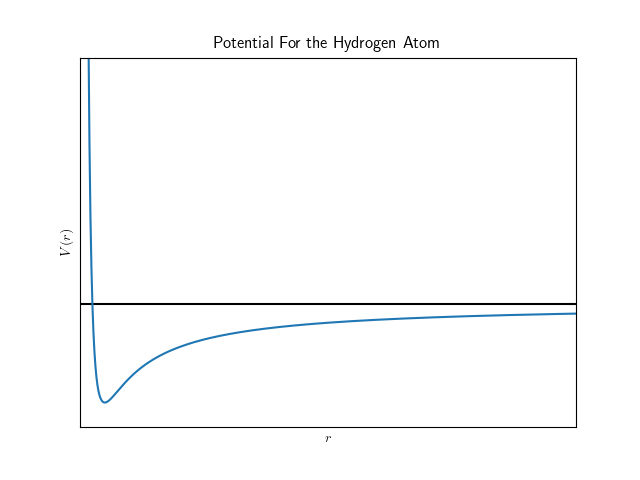
\includegraphics[scale=0.6]{hydrogen_potential.png}
    \caption{The potential for the hydrogen atom.}
    \label{fig:hydrogen atom potential}
\end{figure}

To tidy away even more constants we define
\[a_0 = \frac{\hbar^2}{\mu e^2} \approx \SI{0.52}{\angstrom}, \qquad \text{and} \qquad E_I = \frac{\hbar^2}{2\mu a_0^2} = \frac{\mu e^4}{2\hbar^2} \approx \SI{13.6}{\electronvolt}.\]
\(a_0\) is called the Bohr radius.
We will see the physical significance of these values later.
We now use these quantities to rescale the physical properties of the system:
\[\rho = \frac{r}{a_0}, \qquad\text{and}\qquad \lambda_\ell = \sqrt{-\frac{E_\ell}{E_I}}.\]
Note that since \(E_\ell < 0\) for a bound electron \(\lambda\in\reals\).
We also define \(u_\ell(\rho) = \chi_\ell(\rho)\).
Using this we have
\begin{align*}
    -\lambda_\ell^2E_I\chi(a_0\rho) &= -\lambda_\ell^2E_I u_\ell(\rho)\\
    &= \left[-\frac{\hbar^2}{2\mu}\frac{1}{a_0^2}\dv[2]{\rho} + \frac{\hbar^2\ell(\ell + 1)}{2\mu a_0^2\rho^2} - \frac{e^2}{a_0\rho}\right]\chi_\ell(a_0\rho)\\
    &= \left[-\frac{\hbar^2}{2\mu}\frac{1}{a_0^2}\dv[2]{\rho} + \frac{\hbar^2\ell(\ell + 1)}{2\mu a_0^2\rho^2} - \frac{e^2}{a_0\rho}\right]u_\ell(\rho).
\end{align*}
Which gives us
\[\left[-\frac{\hbar^2}{2\mu}\frac{1}{a_0^2}\dv[2]{\rho} + \frac{\hbar^2\ell(\ell + 1)}{2\mu a_0^2\rho^2} - \frac{e^2}{a_0\rho} + \lambda_\ell^2E_I\right]u_\ell(\rho) = 0.\]
Dividing through by \(-\hbar^2/2\mu a_0^2\) we have
\[\left[\dv[2]{\rho} - \frac{\ell(\ell + 1)}{\rho^2} + \frac{2\mu a_0e^2}{\hbar^2\rho} - \lambda_\ell^2\frac{2\mu a_0^2E_I}{\hbar^2}\right]u_\ell(\rho) = 0.\]
Using the definitions of \(a_0\) and \(E_I\) this becomes
\[\left[\dv[2]{\rho} - \frac{\ell(\ell + 1)}{\rho^2} + \frac{2}{\rho} - \lambda_\ell^2\right]u_\ell(\rho) = 0.\]

\subsubsection{Solution to the Radial Equation}
To motivate an ansatz we will look at the limiting behaviour of the radial equation.
First consider the case that \(\rho \to \infty\), in this case the radial equation reduces to
\[\left[\dv[2]{\rho} - \lambda^2\right]u_\ell(\rho) = 0.\]
The solutions to this are
\[u_\ell(\rho) = e^{\pm\lambda_\ell\rho}.\]
We discard the exponential growth solution as it is non-normalisable so we are left only with the exponential decay solution.
It makes sense for the radial solution to decay exponentially as it becomes increasingly unlikely for the electron to be found as we move away from the proton.
We make the ansatz that
\[u_\ell(\rho) = e^{-\lambda_\ell\rho}\eta_\ell(\rho).\]
Substituting this into the radial equation we have
\begin{align*}
    0 &= \dv[2]{\rho}[e^{-\lambda_\ell\rho}\eta_\ell(\rho)] + \left[\frac{2}{\rho} - \frac{\ell(\ell + 1)}{\rho^2} - \lambda_\ell^2\right]e^{-\lambda_\ell\rho}\eta_\ell(\rho)\\
    &= \dv[2]{\eta_\ell}{\rho}e^{-\lambda_\ell\rho} + 2\dv{\eta_\ell}{\rho}\dv{\rho}e^{-\lambda_\ell\rho} + \eta_\ell(\rho)\dv[2]{\rho}e^{-\lambda_\ell\rho} + \left[\frac{2}{\rho} - \frac{\ell(\ell + 1)}{\rho^2} - \lambda_\ell^2\right]e^{-\lambda_\ell\rho}\eta_\ell(\rho)\\
    &= \dv[2]{\eta_\ell}{\rho}e^{-\lambda_\ell\rho} -2\lambda_\ell 2\dv{\eta_\ell}{\rho}e^{-\lambda_\ell} + \lambda_\ell^2\eta_\ell(\rho)e^{-\lambda_\ell\rho} + + \left[\frac{2}{\rho} - \frac{\ell(\ell + 1)}{\rho^2} - \lambda_\ell^2\right]e^{-\lambda_\ell\rho}\eta_\ell(\rho).\\
\end{align*}
Dividing through by \(e^{-\lambda_\ell\rho}\) we have
\begin{equation}\label{eqn:radial eqn in eta}
    \dv[2]{\eta_\ell}{\rho} - 2\lambda_\ell\dv{\eta_\ell}{\rho} +  \left[\frac{2}{\rho} - \frac{\ell(\ell + 1)}{\rho^2}\right]\eta_\ell(\rho) = 0.
\end{equation}

Now as \(\rho\to 0\) we know from section~\ref{sec:behaviour near the origin central potential} that \(u_\ell(\rho)\sim \rho^{\ell + 1}\).
We expand \(\eta_\ell\) as a power series in \(\rho\) as
\[\eta_\ell(\rho) = \rho^{\ell + 1}\sum_{q = 0}^{\infty} c_q\rho^q.\]
Inserting this into equation~\ref{eqn:radial eqn in eta} we have
\begin{align*}
    0 &= \sum_q \left[(q + \ell + 1)(q + \ell)c_q\rho^{q + \ell - 1} - 2\lambda_\ell(q + \ell + 1)c_q\rho^{\ell + 1} + 2c_q\rho^{q + \ell} - \ell(\ell + 1)c_q\rho^{q + \ell - 1}\right]\\
    &= \sum_q q(q + 2\ell + 1)c_q\rho^{q + \ell - 1} - \sum_q 2(\lambda_\ell[q + \ell + 1] - 1)c_q\rho^{q + \ell}
    \shortintertext{relabelling, \(q \to q - 1\) in the second sum we have}
    &= \sum_q\left[q(q + 2\ell + 1)c_q - 2[\lambda_\ell(q + \ell) - 1]c_{q-1}\right]\rho^{q + \ell - 1}.
\end{align*}
Since we require this to hold for all \(\rho\) we have that for all \(q\)
\begin{equation}\label{eqn:recursion relation}
    q(q + 2\ell + 1)c_q - 2[\lambda_\ell(q + \ell) - 1]c_{q-1} = 0.
\end{equation}
This gives us a recursion relation between the coefficients of the Taylor expansion of \(\eta_\ell(\rho)/\rho^{\ell + 1}\).
For large \(q\) we have
\[\frac{c_q}{c_{q-1}} = \frac{2\lambda_\ell(q + 1) - 2}{q(q + 2\ell + 1)} \to \frac{2\lambda}{q}\]
as \(q \to \infty\) we have
\[c_q \sim c_{q-1}\frac{2\lambda}{q} \sim \frac{(2\lambda_\ell)^q}{q!}.\]
This is the asymptotic behaviour that we expect to give exponential growth in a Taylor series so we expect \(\eta_\ell(\rho) \sim \rho^{\ell + 1}e^{2\lambda\rho}\).
However this is not normalisable.
The only way for this to be normalisable is if for some \(q = n_r\) we have \(c_{n_r} = 0\) as this means that \(c_q = 0\) for all \(q \ge n_r\).
This means that \(\eta_\ell\) is a polynomial of order \(n_r\).
Setting \(q = n_r\) in equation~\ref{eqn:recursion relation} we have that
\[2[\lambda_{n\ell}(n_r + 1) - 1]c_{n_r-1} = 0 \implies \lambda_{n\ell} = \frac{1}{n_r + \ell} = \frac{1}{n}.\]
Here we introduce \(n\), the \define{principle quantum number}.
We see that \(\lambda_{n\ell}\) is quantised as a result of requiring the wave function be normalisable.

\subsubsection{Physical Interpretation}
Since \(\lambda_{n\ell}\) is quantised the energy is also quantised as
\[E_{n\ell} = -\frac{E_I}{(n_r + \ell)^2} = -\frac{E_I}{n^2}.\]
We see that \(E_I\) is the energy needed to remove an electron from the ground state, \(n = 1\).
That is \(E_I\) is the ionisation energy of hydrogen.
Going back to the definition of \(E_I\) we can write
\[E_I = \frac{\mu e^4}{2\hbar^2} = \frac{1}{2}\alpha^2\mu c^2\]
where
\[\alpha = \frac{e^2}{\hbar c^2} = \frac{q^2}{4\pi\varepsilon_0\hbar c} \approx \frac{1}{137}\]
is the \define{fine-structure constant}.
Notice that \(\mu \approx m_e\) and therefore \(\mu c^2\) is approximately the rest energy of the electron.
The energy levels are on the scale of \(\alpha^2\mu c^2/2 \approx \mu c^2 \num{2.7e-5}\).
Since the energy levels are on a scale so much smaller than the rest mass of the electron (which is in turn much less than the rest energy of the proton) we are justified in using a non-relativistic approach.
Any relativistic corrections will typically be \(\order{(\alpha)}\).
Further justification is provided by Heisenberg's uncertainty principle.
Taking \(a_0\) to be a typical length scale in hydrogen we have that \(\Delta p \approx a_0\hbar/2 = \mu e^2/\hbar\).
We can also use the symmetry to state that positive and negative momenta are equally likely so \(\Delta p = \sqrt{\expected{p^2} - \expected{p}^2} = \sqrt{\expected{p^2}}\) from which we have
\[v \sim \frac{p}{\mu} \sim \frac{e^2}{\hbar} = \alpha c \approx \frac{1}{137}c \ll c.\]
So we see that once again relativity only comes into play on scales less than \(a_0\).
Any relativistic corrections are going to be on the order of \(\order{(v/c)} = \order{(\alpha)}\).

We can write the energy levels further as
\[E_n = -\frac{e^2}{2n^2a_0} = -\frac{\mu e^4}{2n^2\hbar^2} = -\frac{\mu q^4}{32\hbar^2\pi^2\varepsilon_0^2n^2}.\]
From \(n = n_r + \ell\) since \(n, n_r\in\naturals_{>0}\) we have that \(\ell = 0, 1, \dotsc, n - 1\), which corresponds to \(n_r = n, n-1, \dotsc, 1\).
For a particular value of \(\ell\) we have \((2\ell + 1)\)-fold degeneracy.
This means that the total degeneracy of the eigenvalue \(E_n\) is
\[g_n = \sum_{\ell = 0}^{n - 1}(2\ell + 1) = 2\sum_{\ell=0}^{n-1}\ell + \sum_{\ell=0}^{n-1}1 = (n - 1)n + n = n^2.\]
Here we have used the result proven in section~\ref{sec:proof sum 0 to n of r is 0.5 n(n+1)}.
The fact that \(E_n = E_I/n^2\) was first proposed by Niels Bohr in 1913 before the full quantum picture that we have seen here was known.
However quantum mechanics is still needed to find the degeneracy of \(E_n\) and other important properties.

The full radial wave function is
\[R_{n\ell}(r) = \frac{\chi_{n\ell}(r)}{r} = \frac{u_{n\ell}(a_0\rho)}{a_0\rho} = \frac{1}{a_0\rho}e^{-\lambda\rho}\eta_{n\ell}(\rho) = \frac{1}{a_0\rho}e^{-\lambda\rho}\sum_{q=0}^{n_r} c_q\rho^{q + \ell + 1}.\]
The polynomials in the last term are called the \define{associated Laguerre polynomials}.
They can be looked up in standard texts.
If we do this we find that
\begin{align*}
    R_{1,0}(r) &= \frac{2}{a^{3/2}}e^{-r/a_0}\\
    R_{2,0}(r) &= \frac{1}{2\sqrt{2}} \frac{1}{a^{3/2}} \left[2 - \frac{r}{a_0}\right] e^{-r/(2a_0)}\\
    R_{2,1}(r) &= \frac{1}{2\sqrt{6}} \frac{1}{a^{3/2}} \frac{r}{a_0} e^{-r/(2a_0)}.
\end{align*}
Notice that \(R\sim a_0^{-3/2}\) so \(\abs{R}^2\sim a_0^3\).
This means that \(\abs{R}\) has units of probability per unit volume, which is what we want since \(\psi = RY_\ell^m\) is a probability density and \(Y_\ell^m\) is dimensionless.

\section{Non-degenerate Time-Independent Perturbation Theory}
Many problems in quantum mechanics involve solving the \gls{tise}.
In most cases however an analytic solution does not exist.
If this is the case then the best we can do is find an estimate.
One of the most common ways to do this is perturbation theory.
This gives us a way to solve the \gls{tise} for a system with a Hamiltonian of the form
\[\operator{H} = \operator{H}_0 + \varepsilon\operator{V}.\]
Here \(\operator{H}\) is the Hamiltonian we wish to find a solution for, \(\operator{H}_0\) is a Hamiltonian for which we know the solution to the \gls{tise} and \(\operator{V}\) is known as a perturbation.
We will assume that \(\operator{H}\) and \(\operator{H}_0\) have discrete, non-degenerate eigenvalues.
Let \(\ket{\varphi_n}\) be the eigenstate of \(\operator{H}_0\) with eigenvalue \(E_n^{(0)}\), i.e.
\[\operator{H}_0\ket{\varphi_n} = E_n^{(0)}\ket{\varphi_n}.\]
We want to find \(\ket{\psi_n}\) and \(E_n\) such that
\[\operator{H}\ket{\psi_n} = E_n\ket{\psi_n}.\]
We look for a solution expanded in terms of \(\varepsilon\).
We can expand the energy as
\[E_n = E_{0n} + \varepsilon E_{1n} + \varepsilon^2E_{2n} + \order{\varepsilon^3} = \sum_{k=1}^{\infty} \varepsilon^kE_{kn},\]
where \(E_{kn}\) are to be found.
Similarly we can expand the eigenstate as
\[\ket{\psi_n} = \ket{\psi_{0n}} + \varepsilon\ket{\psi_{1n}} + \varepsilon^2\ket{\psi_{2n}} + \order{\varepsilon^3} = \sum_{k=1}^{\infty} \varepsilon^k\ket{\psi_{kn}},\]
where \(\ket{\psi_{kn}}\) are to be found.
Inserting these expansions and the definition of \(\operator{H}\) into the \gls{tise} we find that
\[(\operator{H}_0 + \varepsilon\operator{V})\sum_{i=1}^{\infty}\ket{\psi_{in}} = \left[\sum_{j=1}^{\infty}E_{jn}\right]\left[\sum_{k=1}^{\infty}\ket{\psi_{kn}}\right].\]
Expanding these sums up to second order in \(\varepsilon\) we have
\begin{multline*}
    \operator{H}_0\ket{\psi_{0n}} + \varepsilon(\operator{H}_0\ket{\psi_{1n}} + \operator{V}\ket{\psi_{0n}}) + \varepsilon^2(\operator{H}_0\ket{\psi_{2n}} + \operator{V}\ket{\psi_{1n}}) + \order{\varepsilon^3} =\\
    E_{0n}\ket{\psi_{0n}} + \varepsilon(E_{0n}\ket{\psi_{1n}} + E_{1n}\ket{\psi_{0n}}) + \varepsilon^2(E_{0n}\ket{\psi_{2n}} + E_{1n}\ket{\psi_{1n}} + E_{2n}\ket{\psi_{0n}}) + \order{\varepsilon^3}.
\end{multline*}
\subsection{Zeroth Order}
Equating coefficients of terms of zeroth order in \(\varepsilon\) we have
\[\operator{H}_0\ket{\psi_{0n}} = E_{0n}\ket{\psi_{0n}}.\]
Notice that this is exactly what we would get if \(\varepsilon = 0\) so this is just the unperturbed Hamiltonian meaning that \(\ket{\psi_{0n}} = \ket{\varphi_n}\) and \(E_{0n} = E_n^{(0)}\).

\subsection{First Order}
\subsubsection{Energy Perturbation}
Equating coefficients of terms of first order in \(\varepsilon\) we have
\[\operator{H}_0\ket{\psi_{1n}} + \operator{V}\ket{\psi_{0n}} = E_{0n}\ket{\psi_{1n}} + E_{1n}\ket{\psi_{0n}}.\]
Rearranging this we have
\begin{equation}\label{eqn:perturbation theory first order terms}
    (\operator{H} - E_{0n})\ket{\psi_{1n}} - (\operator{V} - E_{1n})\ket{\psi_{0n}} = 0.
\end{equation}
We then take an inner product with \(\ket{\psi_{0n}}\):
\[\bra{\psi_{0n}}\operator{H}_0\ket{\psi_{1n}} - E_{0n}\braket{\psi_{0n}}{\psi_{1n}} - \bra{\psi_{0n}}\operator{V}\ket{\psi_{0n}} + E_{1n}\braket{\psi_{0n}}{\psi_{0n}} = 0.\]
Consider the first term of this sum:
\begin{align*}
    \bra{\psi_{0n}}\operator{H}_0\ket{\psi_{1n}} &= (\bra{\psi_{1n}}\operator{H}_0\hermit\ket{\psi_{0n}})^*\\
    &= (\bra{\psi_{1n}}\operator{H}_0\ket{\psi_{0n}})^*\\
    &= E_{0n}(\braket{\psi_{1n}}{\psi_{0n}})^*\\
    &= E_{0n}\braket{\psi_{0n}}{\psi_{1n}}.
\end{align*}
So the first term cancels with the second, note that we make no assumptions about \(\ket{\psi_{kn}}\) being orthonormal.
Rearranging the remaining two terms we have
\[E_{1n} = \frac{\bra{\psi_{0n}}\operator{V}\ket{\psi_{0n}}}{\braket{\psi_{0n}}{\psi_{0n}}} = \frac{\bra{\varphi_n}\operator{V}\ket{\varphi_n}}{\braket{\varphi_n}{\varphi_n}} = V_{00},\]
where \(V\) is a matrix representation of \(\operator{V}\) and we assume that \(\ket{\psi_n}\) are orthonormal.
Note that since \(E_{0n}\) is a shift in the energy to first order it is sometimes written as \(\Delta E_{0n}\).

\subsubsection{Eigenstate Perturbation}
We can express \(\ket{\psi_{1n}}\) in the energy eigenbasis of \(\operator{H}_0\):
\[\ket{\psi_{1n}} = \sum_{m}c_m\ket{\varphi_m},\]
where as usual \(c_m = \braket{\varphi_m}{\psi_{1n}}\).
We can take a scalar product of equation~\ref{eqn:perturbation theory first order terms} with \(\ket{\varphi_m}\) and we get
\[\bra{\varphi_m}\operator{H}_0\ket{\psi_{1n}} - E_{0n}\braket{\varphi_m}{\psi_{1n}} + \bra{\varphi_m}\operator{V}\ket{\varphi_n} + E_{1n}\braket{\varphi_m}{\varphi_n} = 0.\]
We will first consider the case when \(m \ne n\), thus the last term is zero.
Analogously to how we worked with the first term for the energy perturbation we can show that the first term is simply \(E_{0m}\braket{\varphi_m}{\psi_{1n}}\).
Thus
\[(E_{0m} - E_{0n})\braket{\varphi_m}{\psi_{1n}} + \bra{\varphi_m}\operator{V}\ket{\varphi_n}.\]
Hence
\[c_m = \braket{\varphi_m}{\psi_{1n}} = \frac{\bra{\varphi_m}\operator{V}\ket{\varphi_n}}{E_{0n} - E_{0m}} = \frac{V_{mn}}{E_{0n - E_0m}}.\]
Note that \(E_{0n} = E_n^{(0)}\) and \(E_{0m} = E_m^{(0)}\) are simply the \(n\)th and \(m\)th energy eigenvalues of \(\operator{H}_0\) so are known quantities.
Knowing this we can express the \(n\)th perturbed eigenstate, \(\ket{\psi_{n}}\), as
\[\ket{\psi_{n}} = \ket{\varphi_n} + \varepsilon\sum_{m\ne n}\frac{V_{mn}}{E_{0n} - E_{0m}}\ket{\varphi_m} + \varepsilon c_n\ket{\varphi_n} + \order{\varepsilon^2}.\]
So to find the adjustment needed at first order we just need to compute \(c_n\) which we can do by imposing normalisation, taking the inner product of this with \(\ket{\psi_{n}}\) we have
\[1 = \braket{\psi_{n}}{\psi_{n}} = 1 + 2\varepsilon c_n\braket{\varphi_n}{\varphi_n} + \order{\varepsilon^2},\]
where we have used the fact that \(\ket{\varphi_n}\) are orthonormal so \(\braket{\varphi_n}{\varphi_m} = \delta_{nm}\) meaning that the inner product with the sum term gives zero as \(\ket{\varphi_n}\) is explicitly excluded from that sum.
From this we conclude that we must have \(c_n = 0\), so \(\ket{\psi_{1n}}\) has no component in the \(\ket{\varphi_n}\) direction.
Thus
\[\ket{\psi_{1n}} = \sum_{m\ne n} \frac{V_{mn}}{E_{0n} - E_{0m}}\ket{\varphi_m}.\]

\subsection{Second Order}
Equating coefficients of terms of second order in \(\varepsilon\) we have
\[\operator{H}_0\ket{\psi_{2n}} + \operator{V}\ket{\psi_{1n}} = E_{0n}\ket{\psi_{2n}} + E_{1n}\ket{\psi_{1n}} + E_{2n}\ket{\psi_{0n}}.\]
Rearranging this we have
\[(\operator{H}_0 - E_{0n})\ket{\psi_{2n}} + (\operator{V} - E_{1n})\ket{\psi_{1n}} - E_{2n}\ket{\psi_{0n}} = 0.\]
We then take the inner product with \(\ket{\varphi_n}\) and we have
\[\bra{\varphi_n}\operator{H}_{0}\ket{\psi_{2n}} - E_{0n}\braket{\varphi_n}{\psi_{2n}} + \bra{\varphi_n}\operator{V}\ket{\psi_{1n}} - E_{1n}\braket{\varphi_n}{\psi_{1n}} - E_{2n}\braket{\varphi_n}{\psi_{0n}} = 0.\]
The first term is equal to \(E_{0n}\braket{\varphi_n}{\psi_{2n}}\) so combines with the second term to give zero.
The fourth term is zero as \(\ket{\psi_{1n}}\) has no \(\ket{\varphi_n}\) component.
The scalar product in the fifth term is simply one as \(\ket{\psi_{0n}} = \ket{\varphi_n}\).
Thus
\begin{align*}
    E_{2n} &= \bra{\varphi_n}\operator{V}\ket{\psi_{1n}}\\
    &= \bra{\varphi_n}\operator{V}\sum_{m\ne n} \frac{V_{mn}}{E_{0n} - E_{0m}}\ket{\varphi_m}\\
    &= \sum_{m\ne n}\frac{V_{mn}}{E_{0n} - E_{0m}}\bra{\varphi_n} \operator{V}\ket{\varphi_m}\\
    &= \sum_{m\ne n}\frac{V_{mn}V_{nm}}{E_{0n} - E_{0m}}\\
    &= \sum_{m\ne n}\frac{\abs{V_{mn}^2}}{E_{0n} - E_{0m}}.
\end{align*}

\subsection{Perturbation Examples}
\subsubsection{Infinite Well With a Cosine Floor}
Consider the potential
\[
V(x) = 
\begin{cases}
    V_0\cos\left(\frac{\pi x}{2a}\right), & \abs{x} \le a,\\
    \infty, & \abs{x} > a.
\end{cases}
\]
If we define \(\operator{H}'\) as
\[V_0 \cos\left(\frac{\pi x}{2a}\right)\]
then we can view the Hamiltonian for this system as
\[\operator{H} = \operator{H}_0 + \operator{H}'\]
where \(\operator{H}_0\) is the Hamiltonian for an infinite square well.
The solution to the \gls{tise} for the infinite square well is discussed in section~\ref{sec:infinite square well}.
In particular the \(n\)th energy level is
\[E_n^{(0)} = \frac{\hbar^2\pi^2 n^2}{8ma^2},\]
and the corresponding eigenfunction is
\[
\varphi_{(n)}(x) =
\begin{cases}
    \frac{1}{\sqrt{a}}\cos\left(\frac{n\pi x}{2a}\right), & \text{for odd}~n,\\
    \frac{1}{\sqrt{a}}\sin\left(\frac{n\pi x}{2a}\right), & \text{for even}~n.
\end{cases}
\]
Perturbation theory only gives a good estimate if the energy shift due to the addition of \(\operator{H}'\) to the Hamiltonian is small, in this case this means that we require \(V_0 \ll E_0^{(2)} - E_0^{(1)}\).
The energy shift is then
\begin{align*}
    \Delta E_1 &= \bra{\varphi^{(1)}}\operator{H}'\ket{\varphi^{(1)}}\\
    &= \int_{-a}^{a} \varphi^{(1)}(x)^*V_0\cos\left(\frac{\pi x}{2a}\right)\varphi^{(1)} (x)\dd{x}\\
    &= \frac{V_0}{a} \int_{-a}^{a} \cos^3\left(\frac{\pi x}{2a}\right) \dd{x}\\
    &= \frac{8V_0}{3\pi}.
\end{align*}
So to first order the energy of the ground state is
\[E_1 = E_1^{(0)} + \Delta E_1 = \frac{\hbar^2\pi^2 n^2}{8ma^2} + \frac{8V_0}{3\pi}.\]

\subsubsection{Helium}
Helium is a two electron atom.
If we ignore the interaction between the electrons then the Hamiltonian for a helium atom is
\[\operator{H}_0 = \frac{\hbar^2}{2m}\laplacian_1 - \frac{Ze^2}{r_1} + \frac{\hbar^2}{2m}\laplacian_2 - \frac{Ze^2}{r_2} = \operator{H}_0^{(1)} + \operator{H}_0^{(2)}.\]
Here \(m\) is the reduced mass of an electron and the nucleus,
\[\frac{1}{m} = \frac{1}{m_e} + \frac{1}{2m_p} \approx \frac{1}{m_e}.\]
The distances \(r_1\) and \(r_2\) are the distances from the nucleus to the relevant electron, where we model the four nucleon nucleus as a point charge of charge \(Z = 2e\).
The Laplacian operator, \(\laplacian_1\) or \(\laplacian_2\), acts only on the coordinates of the relevant electron.

The Hamiltonian is independent of the spin of any one part of the system.
This means that we can treat the spin of the electrons as we do for a normal two particle, spin 1, system.
A generic state, \(\ket{\Psi}\in \hilbert\) can be described by \(\ket{\psi}\in\hilbert_{\text{space}}\) and \(\ket{s, s_z}\in\hilbert_{\text{spin}}\) as
\[\ket{\Psi} = \ket{\psi} \tensorProd \ket{s, s_z} = \ket{\psi; s, s_z}.\]
As discussed in section~\ref{sec:total angular momentum}
\[\ket{s=1, s_z=1} = \ket{\spinUp\spinUp}, \qquad \ket{s=1, s_z=-1} = \ket{\spinDown\spinDown}, \qquad\ket{s=1, s_z=0} = \frac{\sqrt{2}}{2}(\ket{\spinUp\spinDown} + \ket{\spinDown\spinUp}),\]
\[\text{and}\qquad \ket{s=0, s_z=0} = \frac{\sqrt{2}}{2}(\ket{\spinUp\spinDown} - \ket{\spinDown\spinUp}).\]
The spatial wave function is given by
\[\braket{\vv{r_1}, \vv{r_2}}{\psi} = \psi(\vv{r_1}, \vv{r_2}) = \psi^{(1)}(\vv{r_1})\psi^{(2)}(\vv{r_2}),\]
where we assume in the last step that a separable solution exists.
Each \(\psi^{(k)}\) must satisfy the \gls{tise} for the relevant Hamiltonian:
\[\operator{H}_0^{(k)}\psi^{(k)}(\vv{r_k}) = \left[\frac{\hbar^2}{2m}\laplacian_k - \frac{Ze^2}{r_k}\right]\psi^{(k)}(\vv{r_k}) = E^{(k)}\psi^{(k)}(\vv{r_k}).\]
This is simply the \gls{tise} that we solved for the hydrogen atom but with the nucleus charge changed to \(Z = 2e\) instead of \(Z = e\).
The solutions to this are the states \(u_{n\ell m}\), where the ground state is
\[\psi^{(k)}(\vv{r_k}) = u_{100}(\vv{r_k}) = \frac{1}{\sqrt{\pi}} \left(\frac{Z}{a_0}\right)^{3/2}e^{-r/a_0}.\]
Thus
\[\braket{\vv{r_1}, \vv{r_2}}{\Psi} = u_{100}(\vv{r_1})u_{100}(\vv{r_2})\sum_{\alpha = 1}^{4}c_\alpha\ket{\alpha}\]
where
\[\{\ket{\alpha}\} = \{\ket{s, s_z}\st s = 0, 1~\text{and}~s_z = -s, \dotsc, s\}.\]
Electrons are fermions.
This means that \(\ket{\Psi}\) should be antisymmetric under exchanging of 1 and 2.
The radial part, \(u_{100}(\vv{r_1})u_{100}(\vv{r_2})\), is symmetric under exchanging of 1 and 2 so the spin part must be antisymmetric.
The only antisymmetric spin state available is \(\ket{s = 0, s_z = 0}\).

We are now in a position to consider what happens when we include the interaction between the electrons.
This interaction is characterised by the potential
\[\operator{V} = \frac{e^2}{\abs{\vv{r_1} - \vv{r_2}}}.\]
The energy shift due to this perturbation is
\begin{align*}
    \Delta E_1 &= \bra{\Psi}\operator{V}\ket{\Psi}\\
    &= \bra{\psi; 0, 0}\operator{V}\ket{\psi; 0, 0}
    \shortintertext{using the fact that \(\operator{V}\) acts only on the radial part this becomes}
    &= \braket{0, 0}{0, 0}\bra{\psi}\operator{V}\ket{\psi}
    \shortintertext{considering the ground state, \(\psi(\vv{r}) = u_{100}(\vv{r})\), or equivalently \(\ket{\psi} = \ket{100}\), this becomes}
    &= \bra{100, 100}\operator{V}\ket{100, 100}\\
    &= \int \dd[3]{r_1}\dd[3]{r_2} u_{100}^*(\vv{r_1})u_{100}^*(\vv{r_2})\frac{e^2}{\abs{\vv{r_1} - \vv{r_2}}}u_{100}(\vv{r_1})u_{100}(\vv{r_2})\\
    &= \left(\frac{eZ^3}{\pi a_0^3}\right)^2 \int \dd[3]{r_1}\dd[3]{r_2} \exp\left(-\frac{2Z(r_1 + r_2)}{a_0}\right)\frac{1}{\abs{\vv{r_1} - \vv{r_2}}}\\
    &= \frac{5}{4}ZE_I
\end{align*}
where \(E_I \approx \SI{13.6}{\electronvolt}\) is defined as it was in section~\ref{sec:stationary states hydrogen atom}.